\documentclass[11pt,a4paper]{report}
\usepackage[francais]{babel}%
\usepackage[T1]{fontenc}% 
\usepackage[utf8x]{inputenc}
\usepackage{amsmath}
\usepackage{graphicx}
\usepackage{hyperref}
\usepackage{setspace}
\usepackage{tabularx}
\usepackage{array}
\usepackage[toc,page]{appendix}
\renewcommand\thesection{\arabic{section}}

\begin{document}
\newcolumntype{M}[1]{>{\raggedright}m{#1}}
\linespread{0.99}
\hyphenpenalty=750

\date{05 Septembre 2016}
\newcommand{\mydate}{\formatdate{4}{7}{2016}}

\begin{titlepage}
\newcommand{\HRule}{\rule{\linewidth}{0.5mm}}
\centering

\textsc{\large \textbf{Université Paris Ouest Nanterre La Défense}}\\[1.5cm] % Name of your university/college

% * <lhillah@u-paris10.fr> 2016-08-17T09:04:55.535Z:
%
% > 
\includegraphics[]{upond.PNG}\\
%
% Logo doit être moins plus discret dans le placement, pas en plein milieu.
%
% ^.
\textsc{\large Mémoire de Master 2 MIAGE}\\[0.5cm] % Major heading such as course name
\textsc{\large Département Mathématiques et Informatique}\\[0.5cm] % Major heading such as course name
\textsc{\large UFR SEGMI}\\[0.5cm] 
\HRule \\[0.4cm]
{ \large  \textbf{Le Data Mining}:\\ Application des techniques de Data Mining aux données clients pour améliorer la gestion des risques  dans la finance de marché du secteur de l'énergie}\\[0.4cm] % Title of your document
\HRule \\[1cm]
\emph{Soutenu par \textbf{Moussa KANOUTE}}\\ le 05/09/2016\date{04 Juillet 2016}\\[1cm]
\large En vue de l'obtention du grade de Master de l'université Paris Ouest Nanterre La Défense
\\[1cm]
\begin{minipage}{0.4\textwidth}
\begin{flushleft} \large
\emph{Responsable de la filière Miage par voie classique:} \\
Pr \textbf{Pascal Poizat} % Supervisor's Name

\end{flushleft}
\end{minipage}
~
\begin{minipage}{0.4\textwidth}
\begin{flushright} \large
\emph{Tuteur enseignant:}\\
Dr \textbf{Lom HILLAH}\\
\emph{Tuteur entreprise:}\\
M \textbf{Eric STOLL}, Pilote risque de crédit chez EDF
\end{flushright}
\end{minipage}\\[2cm]
\date{05 Septembre 2016}

\vfill

\includegraphics[width=3cm]{upond.PNG} 
\hfill 

\includegraphics[width=3cm]{logo_edf_carre.png} 
\end{titlepage}

~
\thispagestyle{empty}
\newpage
% * <lhillah@u-paris10.fr> 2016-08-17T08:24:30.522Z:
%
% Ceci n'est pas un vrai résumé. Un résumé doit donner un aperçu synthétique du contexte, de la problématique et votre contribution.

 
%
% ^.
% * <babakanoute@gmail.com> 2016-08-17T12:41:27.703Z:
%
% OK
%
% ^.
\begin{abstract}

Depuis l'ouverture du marché de l'énergie à la concurrence en 2007, les acteurs du secteur de l'énergie sont en train de mettre en place de nouvelles stratégies pour adapter leurs offres et répondre aux besoins des clients. Cependant, se positionner comme leader sur un marché ouvert à la concurrence impose une remise en question de ses besoins. Par exemple, chez EDF, le groupe met l'accent sur l'innovation et le développement.\\\\ L'un des enjeux actuels des acteurs de l'énergie est la réduction des pertes et des impayés liés aux clients professionnels. Il s'agit d'anticiper et de réduire les risques de non-paiement de manière efficace tout en évitant les procédures judicaires qui peuvent engendrer des coûts non négligeables. \\\\
L'objectif de ce mémoire est d'étudier et d'appliquer les techniques de Data Mining au sein de la finance de marché du secteur de l'énergie, plus précisément les risques liés aux clients. Il s'agit des clients grands comptes (importantes sociétés industrielles) jusqu'aux petites entreprises. Nous allons tenter de mettre en place de façon efficace une autre approche de la gestion des données clients à travers des outils de Data Mining dont nous disposons.     


% * <lhillah@u-paris10.fr> 2016-08-17T08:23:05.045Z:
%
% > L'essor actuel du Data Mining aussi bien dans le monde industriel qu'universitaire où il est l'objet d'enseignement et de recherche est en plein développement\cite{resume}
%
% Cette phrase n'a pas beaucoup de sens... (l'essor ... est en plein développement)
%fait
% ^.
\end{abstract}
\newpage
\section*{Remerciements}
\thispagestyle{empty}
Avant d’entamer la présentation de ce travail, je voudrais d’abord adresser mes sincères remerciements et reconnaissances à tous ceux qui m’ont, si efficacement, aidé à effectuer
mon alternance dans de bonnes conditions.\\

En particulier, à mon tuteur en entreprise, Monsieur Eric STOLL, souhaitant qu’il trouve ici l’expression de ma profonde reconnaissance pour sa disponibilité, ses critiques et ses précieux conseils qu’il m’a accordé tout au long de ce travail.
Mes remerciements vont également à tous les membres de l’équipe Credit Management.\\

Je souhaite aussi remercier mon tuteur enseignant, Monsieur Lom HILLAH pour ses précieux conseils et son assistance. Je  remercie également l’ensemble de l’équipe pédagogique qui nous a suivis tout au long de cette dernière année de master MIAGE.\\

Enfin, j'adresse mes remerciements à mes parents pour leurs sacrifices, leurs confiances et tout le soutien qu'ils m'ont accordé tout au long de mes études. \\
 




\newpage
\setcounter{page}{1}
\section*{Introduction}


Pour mieux comprendre les besoins des entreprises en matière d'énergie, les fournisseurs doivent adapter leurs stratégies au comportement des clients. Face à l'évolution de la technologie, les acteurs fournisseurs et distributeurs d'énergie modifient leurs environnements analytiques dans le but de perfectionner leurs outils d'analyse, de mettre au point des solutions de produits et services adaptés à chaque type de client.\\

Face à des contraintes budgétaire et réglementaire de plus en plus fortes, le secteur de l'énergie doit innover pour gagner en productivité et adapter leurs offres par rapport aux prix du marché, revoir leurs politiques de ventes où ils doivent pouvoir maîtriser les dépenses pour réduire les coûts et réduire l'impact sur l'environnement. \\

Les entreprises ont besoin de connaître dans un premier temps le processus réel des métiers. Cela permet d'identifier tous les éléments potentiels dans un objectif d'amélioration continue de la qualité. Par la suite, nous pouvons appliquer à ces processus des techniques ou des méthodes permettant de prendre des décisions.
De nos jours, les entreprises sont confrontées à une multitude de données diverses. Ces données ne sont pas toujours cohérentes les unes avec les autres (Excel, base de données relationnelle, sources externes, outils comptables ...). Certaines données mesurent des faits qualitatifs et quantitatifs et sont sous exploitées. Ces données représentent des informations capitales pour les entreprises notamment pour appréhender les processus métiers dans leur globalité.\\
Ce sujet m'intéresse car durant mon alternance je me suis rendu compte de la complexité du traitement des données. La récupération et le traitement d'énormes masses de données relèvent d'enjeux fonctionnels et stratégiques. \\
Notre contribution consiste à améliorer la gestion des risques client en s'appuyant sur des techniques de Data Mining avec un apprentissage dirigé et non dirigé.\\ 

Ce mémoire se compose de 7 chapitres. Dans le chapitre \ref{chap1} nous parlerons du contexte actuel lié au Data Mining et énoncerons la problématique. Ensuite, les chapitres  \ref{etat_de_lart}  et \ref{concept_et_technique}, nous présenterons l'état de l'art en illustrant les utilisations actuelles, les problèmes liés au Data Mining, les concepts et les techniques. Dans les chapitres \ref{demarche} et \ref{mise_en_oeuvre}, nous allons mettre en place la démarche à appliquer par rapport à notre problématique et allons tenter de mettre en œuvre la solution en combinant plusieurs approches et en les appliquant à notre problème. Dans le chapitre \ref{bilan}, nous allons faire un bilan des résultats obtenus (avantages et limites). Enfin, dans le chapitre \ref{conclusion} nous terminerons notre étude par la conclusion. 

\newpage

\tableofcontents
\thispagestyle{empty}
\newpage
\listoffigures
\newpage
\listoftables
\newpage
\section{Contexte et problématique \label{chap1}}
Dans ce chapitre, nous allons tout d'abord parler du contexte, ensuite nous expliquons le problème que nous allons tenter de résoudre. 
\subsection{Contexte}
Le secteur de l'énergie connaît une forte concurrence entre les différents acteurs. Autrement dit, comment un géant historique de l’énergie peut-il résister aux nouveaux entrants agiles qui donnent la priorité à des services à forte valeur proposée, à un tarif particulièrement concurrentiel ? "\textit{Cette concurrence s'inscrit dans un contexte qui exige de multiples changements de modèles économiques conclus par la transition énergétique tels que : une production décentralisée, la gestion complexe du réseau électrique avec une part croissante de renouvelable (smart grids), la gestion de la demande, une meilleure connaissance des clients grâce à l’exploitation des données (Data Mining) qui seront fournies par les compteurs intelligents, une nouvelle relation client, des objets connectés, etc}" \cite{cap}. 
Pour qu'une entreprise arrive à faire face à ces problèmes et assurer une stabilité financière, il est nécessaire pour elle d'innover et de mettre en place de nouvelles actions telles que  des actions sur les créances clients pour limiter ou contrôler les délais de règlement, tout en surveillant de près la santé financière des clients. La Figure  \ref{figure1} montre le rapport des délais de paiements des entreprises (Source: infolegale) \cite{infolegale}.   
\begin{figure}[h]
   \centering
   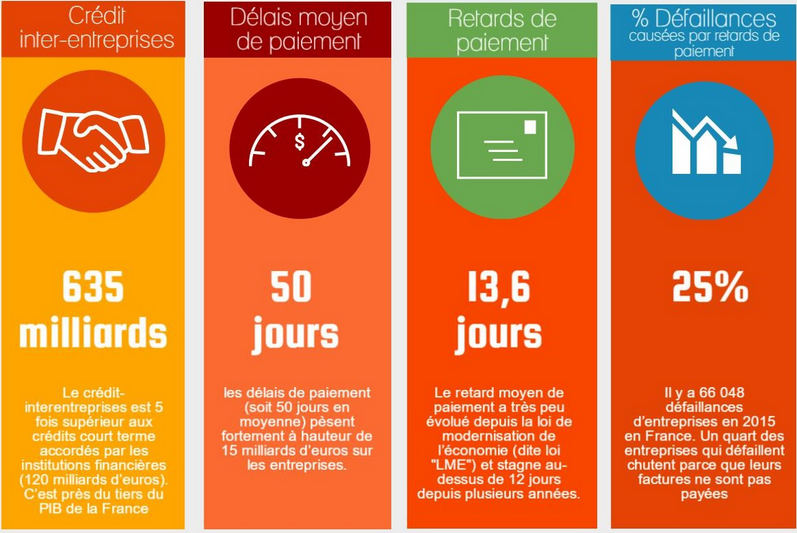
\includegraphics[scale=0.50]{infolegale.PNG}
      \caption{Rapport 2015 de l'observatoire des delais de
      paiement}
      \label{figure1}
\end{figure}

On voit clairement les enjeux sur la gestion des risques clients, d'où l'intérêt de disposer des moyens efficaces pour anticiper ces risques. En 2015, un quart des entreprises fait faillite  pour cause de retards de paiement.

\newpage
\subsection{Problématique}
Supposons qu’une mine d’or possède 20\% d’or visuel et que le reste (80\%) se trouve sous terre. Une exploitation minière est nécessaire pour extraire toute ou partie de l’or. Il s'agit d'exploiter toutes les ressources dont nous disposons pour répondre rapidement aux problèmes et anticiper des actions futures. 
Dans un contexte informatique il s’agit d’avoir les moyens à disposition afin d’avoir une meilleure visibilité sur l’ensemble des données à travers des techniques et des méthodes adaptées aux métiers. 
\subsection*{Comment exploiter efficacement les données pour améliorer la gestion des risques liés aux clients dans le secteur de l’énergie ?}

L’une des solutions est le Data Mining, car qu’il favorise la mise en place d'algorithmes capables d'exploiter rapidement et intelligemment des informations nouvelles et utiles permettant aux utilisateurs de mieux orienter leurs actions. Il permet aussi de réduire les temps de production (traitements, exploration, analyses…) des données et d’automatiser un certain nombre de d'opérations liées aux règles de gestions.\\\\
Par ailleurs, la plupart des outils proposant des solutions de Data Mining ne sont pas auto suffisants, c’est-à-dire qu'une personne qui ne connaît pas le métier ne pourrait pas interpréter les résultats fournis par les outils de Data Mining.\\\\
 Les méthodes d'analyses appliquées aux clients à risque se font de façon manuelle. Par exemple pour évaluer une entreprise, c'est à la fois la recherche d'information issue de plusieurs outils et l'application de la politique de risque. \\

A ce jour, l'approche actuelle se résume à la gestion manuelle des portefeuilles clients. Toutes les situations d'impayés ne sont pas traitées, c'est à dire les analystes se fixent un seuil qui pourrait être par exemple les clients avec un montant d'impayé élevé. On constate très vite que tous les cas ne sont pas traités. Les clients ne faisant pas parties de ce seuil ne sont pas surveillés ou laissés tels qu'ils sont jusqu'à ce que les analystes les détectent autrement. Notre démarche consiste à mettre en œuvre une nouvelle approche qui est de proposer une autre façon de traiter les données pour résoudre ces besoins qui, aujourd'hui sont nécessaires pour améliorer la gestion des risques de crédit et anticiper les pertes futures. Cette approche est intéressante dans le sens où elle permet d'avoir une vue globale de tous les clients en situation d'impayés mais aussi d'anticiper et prévenir des cas délicats qui sont difficilement détectables par l'approche actuelle.
 \\
% * <lhillah@u-paris10.fr> 2016-08-17T09:12:36.719Z:
%
% > Notre démarche consiste à mettre en œuvre les techniques de Data Mining pour résoudre ces besoins qui, aujourd'hui sont nécessaires pour améliorer la gestion des risques de crédit et anticiper les pertes.
%
% On ne présente pas une démarche, une solution dans une section problématique avant d'avoir énoncé clairement le problème !
%
% ^.
% * <babakanoute@gmail.com> 2016-08-17T13:11:10.847Z:
%
% OK
%
% ^.

Dans ce chapitre nous allons parler de la manière dont les données sont traitées et analysées actuellement. Il s'agit de traiter l'ensemble des données clients 
% * <lhillah@u-paris10.fr> 2016-08-17T09:13:30.809Z:
%
% > Dans ce chapitre nous allons parler de la manière dont les données sont traitées et analysées actuellement. Il s'agit de traiter l'ensemble des données clients 
% > et non un échantillon de celles ci pour identifier des sources de valeur pour l'entreprise. Les applications de traitement de données sont le plus souvent destinées à fournir des données brutes. Ces données sont collectées pour produire des analyses où encore des tableaux de bord qui conduisent à des résultats réels. \newline
%
% Vous êtes déjà en train d'annoncer votre démarche avant d'expliquer le problème...
%
% ^.OK
et non un échantillon de celles-ci pour identifier des sources de valeur pour l'entreprise. Les applications de traitement de données sont le plus souvent destinées à fournir des données brutes. Ces données sont collectées pour produire des analyses où encore des tableaux de bord qui conduisent à des résultats réels. \newline
  

% * <lhillah@u-paris10.fr> 2016-08-17T09:14:06.404Z:
%
% > Supposons qu’une mine d’or possède 20\% d’or visuel et que le reste (80\%) se trouve sous terre. Une exploitation minière est nécessaire pour extraire toute ou partie de l’or. Dans un contexte informatique il s’agit d’avoir les moyens à disposition afin d’avoir une meilleure visibilité sur l’ensemble des données à travers des techniques et méthodes adaptées aux métiers. 
%
% C'est anecdotique. On peut tolérer cela juste comme premier paragraphe de cette section. Mais tout de suite après, il faut présenter le problème de manière plus sérieuse, quitte à se focaliser immédiatement sur le secteur de l'énergie, votre domaine d'application.
%
% ^.

A ce jour, il existe des solutions classiques permettant de résoudre partiellement ce problème. Il s’agit des outils traditionnels (Tableur, Base de données classiques…).\\

Pour permettre aux analystes d’accéder aux données massives, il existe un besoin qui est de mettre à disposition l'ensemble des données à travers des outils de traitement à la fois simples et efficaces. Cela leur permet d’agir plus vite en prenant des décisions et en identifiant des anomalies clients par exemple. \newline

\subsubsection{Les problèmes liés aux données}
La préparation des données est une des premières étapes du Data Mining. Cette étape permet de constituer une base d'analyse de données qui servira pour le test. Elle pose quelques difficultés vis-à-vis des types de données, la valeur et la taille.
En effet, l'absence des données n'est pas compatible avec tous les outils de gestion des données. Dans ce cas, soit on exclut les enregistrements incomplets soit on remplace les données manquantes.\\ 
Il est rare que les données disponibles soient directement opérationnelles. Très souvent, il faut au préalable transformer ces données pour permettre aux outils de Data Mining un traitement plus facile. L’étape de transformation peut varier selon la technique et les outils. Par exemple un système qui fonctionne en COBOL code les textes stockés en EBCDIC\footnote {EBCDIC : C'est un mode de codage des caractères sur 8 bits créé par IBM à l'époque des cartes perforées} et les nombres en « décimal condensé », tandis que les systèmes d’aide à la décision et les applications d’exploitation de données utilisent d’autres langages qui codent les textes à stocker en ASCII et les nombres comme des entiers ou en virgule flottante simple... (Gordone linoff) \cite{concepts}. Notre base est constituée à la fois de variables continues, discrètes, qualitatives et quantitatives.\\

 
\subsubsection{Motivation}
Ayant un intérêt dans le traitement, la gestion et l'analyse des données, j'ai décidé d’approfondir mes connaissances dans la fouille des données. Ce domaine est un élément essentiel pour les systèmes d'aides à la décision dans le monde des entreprises.    
Le choix de mon sujet s'explique par ma curiosité à traiter des données massives à travers différentes applications. J'ai appris lors de mon alternance chez EDF des enjeux et des difficultés liées à la gestion des données. Cela m'a permis de prendre du recul tout en essayant de comprendre les besoins du métier et les objectifs afin d'aider à tirer parti de toute cette complexité.  



\newpage

\section{Etat de l'art \label{etat_de_lart}}
% * <lhillah@u-paris10.fr> 2016-08-17T08:40:32.074Z:
%
% > Etat de l'art
%OK
% ^.
Aujourd'hui, les industries qui utilisent les grands volumes de données comme les services de production, les services financiers, les télécommunications et les assurances sont soumises à une accélération significative de la concurrence. Les entreprises de ces secteurs riches en informations disposaient depuis longtemps des données et les ressources demandées par le Data Mining.
 Nous soulignons toutefois que les techniques et outils décrits s'appliquent dans d'autres domaines comme dans le domaine de l'assurance, de la télécommunication... \\\\
 Dans cette partie, nous allons exposer quelques exemples d'utilisations du Data Mining par secteur. Ensuite, nous allons comparer l'utilisation du Data Mining dans le secteur de l'énergie par rapport aux autres secteurs. 
 Nous présentons également les différents outils qui peuvent répondre à notre objectif et les comparons à travers des exemples selon les mêmes critères. 


 \subsection{Le Data Mining par secteur}
 Depuis plusieurs années, le Data Mining est utilisé dans plusieurs secteurs. Dans cette section, nous citons quelques secteurs d'applications qui intègrent les techniques de Data Mining dans leurs tâches quotidiennes. 
\subsubsection{Le secteur bancaire}
% * <lhillah@u-paris10.fr> 2016-08-17T08:28:30.428Z:
%
% > Le secteur bancaire
%
% C'est faible. Vous n'expliquez pas ce que c'est que le scoring. Vous n'expliquez pas en ce qu'apporte les techniques de DM au secteur bancaire et sur quels problèmes ces techniques étaient appliquées.
% OK
% ^.
  C'est dans le secteur bancaire qu'est né le scoring de risque\footnote{Scoring de risque: Le scoring est une technique qui permet d’affecter un score à un client ou prospect}, au milieu du 20ème siècle, à une époque où les calculs étaient simplistes \cite{stephane}. Les analystes  conçoivent à cet effet des grilles de scores par analyse, sur le passé, des corrélations entre la situation initiale déclarée des clients et les événements survenus.
   De multiples techniques du Data Mining comme le scoring, la classification, l'association des produits se sont étendus dans la banque de détail et la banque d'entreprise. \\\\
 Dans le cadre de la lutte contre la fraude, les opérations de trading génèrent un nombre important de données. Le Data Mining en quasi-temps réel va aider à éviter les fraudes en analysant les données du marché ainsi que les comportements des traders. C'est ainsi que la Société générale CIB optimise sa gestion de risques depuis l'affaire Kerviel \cite{banque_fraude}.\\ La société de paiement en ligne PayPal utilise la solution Terracota de l'éditeur allemand Software AG qui calcule la corrélation en temps réel afin d'identifier des dysfonctionnements et donner lieu à des corrections immédiates. Cette recherche a permis à PayPal de passer de 50 à 1 000 règles de contrôle antifraude entre le clic et le paiement, c'est-à-dire en moins de 650 millisecondes d'après Christian Lefèvre, directeur de la branche banque et assurance chez Software AG France \cite{banque_fraude}.\\\\ 
  Cependant, les banques s'orientent de plus en plus vers l'usage du Data Mining en temps réels pour lutter contre la fraude. Il s'agit de fouiller des millions de données en temps réels or les accès aux données à travers différents systèmes dans le secteur bancaire reste un frein en terme de protection des données clients. L'application du Data Mining montre ces limites dans ce genre d'opérations.
 

  \subsubsection{Le secteur de l'assurance}
 L'une des forces des acteurs de l'assurance 
 réside dans l'expérimentation des analyses prédictives. L'analyse prédictive a pour objectif d'associer une probabilité à une action future. 
  Le secteur de l'assurance connaît  une forte utilisation de Data Mining pour relever différents défis. L'importance de l'exploitation des données dans le secteur de l'assurance est primordiale. \\\\
  Comme l’explique Thomas H. Davenport \cite{thomas} dans le Harvard Business Review, l’analyse prédictive n’est pas une idée neuve dans le monde de l’entreprise. Dans le secteur de l’assurance, les actuaires utilisent quotidiennement des données du passé et construisent des modèles analytiques. Les résultats obtenus via ces modèles statistiques servent directement à la prise de décision. L’assurance a ainsi été l'un des premiers secteurs à utiliser l’analyse prédictive dans la gestion du risque client via des méthodes de scoring \cite{Benjamin}.\\\\
  Les compagnies d'assurance perdent beaucoup d'argent chaque année à cause d'indemnisation frauduleuse. Pour identifier ces cas, ils se servent des techniques de Data Mining dans leurs processus de vérification. Durant le processus d'indemnisation, les dossiers des clients sont scorés de façon automatique sur des problématiques de détection de fraude, de calcul de provisions, de recouvrement ou encore pour estimer la complexité des dossiers. Ce procédé se déroule en continu et en parallèle du traitement de la déclaration de sinistre permettant une actualisation permanente de l’évaluation du risque. Selon The Economist, le fait d'automatisé le scoring sur les dossiers clients réduirait de 90\% les frais de souscription \cite{assurance_fraude}.\\\\ 
 Il existe cependant des tendances qui remettent en cause les modèles prédictifs des acteurs de l'assurance. Parmi ces tendances, on peut citer la variation de la nature des risques. Lorsque les risques évoluent dans le temps, ils obligent les acteurs à repenser leurs modèles et à adapter leurs méthodologies de façon pertinente.\\  Une autre limite est le risque dont on ne connait pas la probabilité de survenance. Il est difficile d'intégrer ce genre de risque dans le modèle prédictif. Un exemple de cas est lorsqu'une personne souscrit à un contrat, il est possible qu'il change de comportement et prend plus de risque.  
 
  
% * <lhillah@u-paris10.fr> 2016-08-17T08:31:21.980Z:
%
% > Une étude a été menée par IBM en 2010 \cite{ibm} sur l'utilisation du Data Mining pour détecter la fraude à l'assurance.
%
% Quand on mentionne une étude, il faut expliquer ses résultats.
% OK
% ^.
 
   
% * <lhillah@u-paris10.fr> 2016-08-17T08:30:32.492Z:
%
% > l’analyse prédictive 
%
% Analyse prédictive pas introduite; ça sort de nulle part.
% OK
% ^.

 \subsubsection{Le secteur de la grande distribution}
 
 La grande distribution utilise le Data Mining  pour mieux connaître les profils de leurs clients en tenant compte de plusieurs facteurs. Un exemple de cas pratique est l'étude des tickets de caisse. Les informations sur les tickets de caisse permettent d'identifier les profils clients, de mieux choisir les produits et de les disposer dans les rayons. \cite{stephane})
 
 \subsubsection{Le secteur de l'automobile}
Depuis l’arrivée des voitures autonomes, l'industrie automobile entre dans une nouvelle ère. Pour des raisons de sécurités, ces voitures autonomes sont dotées de capteurs pour collecter des données. Ces données peuvent permettre de prédire des pannes avant qu’elles ne surviennent. L’utilisateur peut solliciter l’intervention d’un technicien avant d’être confronté à un problème \cite{auto_mining}. C’est la maintenance prédictive. 
Le champ d'application du Data Mining dans le secteur automobile est large. Un thème classique est le score de rachat d'un véhicule de la marque. Dans son ouvrage "Data Mining et statistique Décisionnelle", Stéphane TUFFERY explique que Renault a ainsi construit un modèle prédisant les clients susceptibles d'acheter un nouveau véhicule Renault dans les six mois à venir\cite{stephane}. \\
Une autre application possible du Data Mining est l’analyse des données de consommation de carburant. Les informations correspondantes sont recueillies par les instruments du tableau de bord et peuvent également être présenté au conducteur. Dans le cas des véhicules internes d’essai et de pré production, ces données sont enregistrées et conservées afin de pouvoir établir des comparaisons de la consommation d’un pays à l’autre \cite{bmw}.

\newpage
 \subsubsection{Le secteur de la téléphonie mobile}
 Les compagnies de télécommunications génèrent une importante quantité de données. Ces compagnies se servent du Data Mining pour identifier par exemple des appels téléphoniques frauduleux ou les défauts de réseaux.
 Les enregistrements d'appels comprennent des informations suffisantes pour décrire les caractéristiques importantes de chaque appel. Au minimum, chaque enregistrement d'appel comprend les numéros de téléphone émetteur et récepteur, la date et l'heure de l'appel et la durée de l'appel.  La figure \ref{telephone} ci-dessous compare la moyenne d'appels par semaine entre les entreprises et les particuliers. Entre neuf heures du matin et quatre heures du soir les entreprises émettent 1.5 fois plus d'appels que les particuliers dans la semaine. Cette étude a été menée par Cortes et Pregibon en 2001 dans le cadre de la distinction du type de profil client qui émet le plus d'appel (en termes de pourcentage) dans la semaine. \cite{tekephone_secteur} 

% * <lhillah@u-paris10.fr> 2016-08-17T08:34:50.005Z:
%
% >  La figure 
%
% Donner un label à la figure, et la référencer dans le texte, avec \ref{}. Il faut citer la source de cette figure et dans quel contexte d'étude ça a été produit
%
% ^. OK 
 \begin{figure}[h]
   \centering
   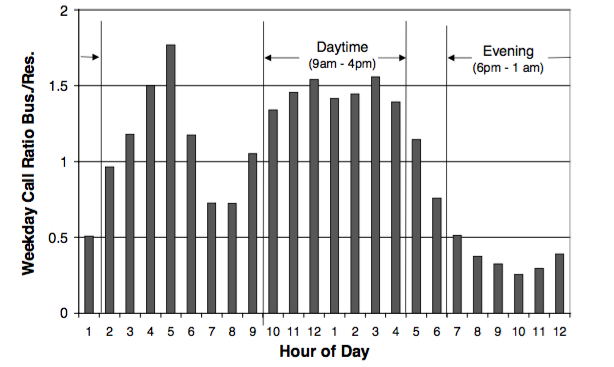
\includegraphics[scale=0.5]{telephone.png}
      \caption{Rapport du temps d'appel par semaine entreprise/Residence}
      \label{telephone}
\end{figure}


% * <lhillah@u-paris10.fr> 2016-08-17T08:36:27.679Z:
%
% > Dans son ouvrage
%
% Donner le titre de l'ouvrage, même si on a la référence bibliographique 12.
% OK 
% ^.


\subsubsection{Le secteur de la santé}
Le Data Mining est très souvent utilisé dans le domaine de la santé depuis plusieurs années. Dans un article publié en 2013, il est prouvé que le Data Mining améliore les prescriptions médicales \cite{medecine}. Le Data Mining aide à réaliser les objectifs de diagnostic, de traitement des patients. 
En effet les chercheurs de Stanford ont analysé des millions de dossiers sur les patients et ils ont élaboré une méthode adaptée aux dossiers analysés, essentiellement composés de texte. Une première qui ouvre la porte à des analyses poussées. La difficulté du projet tenait à ce que la grande majorité des informations pertinentes pour une telle étude était sous forme de textes dans les notes prises par les médecins. Les chercheurs ont donc établi une liste de mots-clés qu’ils ont utilisé pour fouiller dans les dossiers identifiés comme potentiellement à risque.


% * <lhillah@u-paris10.fr> 2016-08-17T08:39:00.004Z:
%
% > Le Data mining est très souvent utilisé dans le domaine de la santé depuis plusieurs années. Dans un article publié en 2013, il est prouvé que le Data Mining améliore les prescriptions médicales \cite{medecine}. En effet les chercheurs de Stanford ont analysé des millions de dossiers sur les patients et ils ont élaboré une méthode adaptée aux dossiers analysés, essentiellement composés de texte. 
%
% Comment cela fut-il mis en oeuvre en pratique ?
%	OK
% ^.

\subsubsection{Le secteur de l'énergie}

Depuis 2010, ENEDIS (anciennement appelé ERDF) la filiale du groupe EDF s'est lancé dans le projet des compteurs communicants appelés compteurs Linky \footnote{Linky: C'est un compteur communicant, c'est-à-dire qu'il échange des données automatiquement avec un centre de contrôle}. Selon ENEDIS, \textit{Linky présente de nombreux avantages pour le client. À commencer par une facture qui pourra être calculée sur la base de la consommation réelle, des interventions réalisées à distance (donc sans contrainte de rendez-vous) et dans des délais beaucoup plus courts} \cite{linky}.\\\\
Lorsque les données sont collectées et transmises par Linky au système d'information, ENEDIS dispose d'un outil d'analyse qui permet d'exploiter, de traiter, de croiser et de mettre à disposition des parties prenantes. Un exemple de cas d'utilisation est l'intégration de l'ensemble des données réseaux pour réaliser des études réseaux ENEDIS et anticiper le dimensionnement du futur réseau public de distribution. \\\\
Les données collectées sont également utilisées par différents outils d’analyse et de traitement statistique en vue de la reconstitution des flux pour les marchés de l’électricité. Grâce à des outils spécifiques dit de « Data Mining », elles permettent par exemple de construire des profils type, d’identifier les pertes non techniques potentielles ou d’élaborer des méthodes d’évaluation de l’effacement via des panels de consommateurs \cite{linky2}.

 La figure \ref{enedis} montre un exemple d'évolution de courbes de charge de consommation à travers des données provenant du compteur Linky en 2015.
\newpage

 \begin{figure}[h]
   \centering
   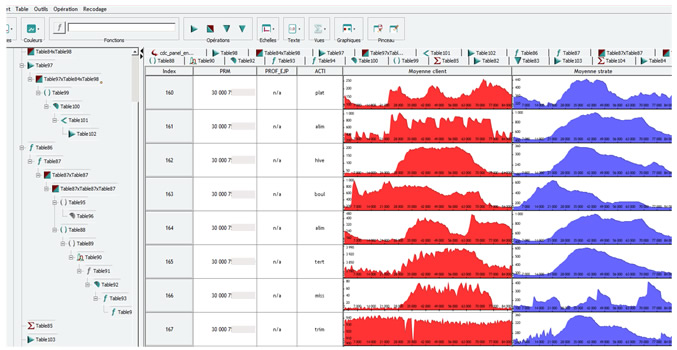
\includegraphics[scale=0.5]{enedis.jpg}
      \caption{Exemple d'analyse de courbes de charge de consommation - Source: ENEDIS}
      \label{enedis}
\end{figure}


Après les compteurs communicants, nous allons parler des bâtiments connectés en terme d'analyse de données pour une connaissance fine de la demande et de la consommation. Il permet d’adopter des solutions efficaces de gestion en installant des capteurs et compteurs connectés, de jouer sur la qualité du bâtiment (isolation, inertie thermique, etc.), le choix des équipements (production d’énergie, distribution, rendement) est de penser en terme d’efficacité énergétique active (optimisation, lutte anti-gaspillage, sensibilisation des usagers) \cite{batiment}. Il existe de plus en plus de solutions logicielles pour centraliser les données de plusieurs bâtiments comme la société Intent Technology \footnote{Intent Technology: Société spécialisée dans la transformation numérique des bâtiments connectés}.\\\\
 Mise à part la collecte et le stockage des données, il existe un autre défi qui est de disposer des outils d'analyses. En effet, cela est plus compliqué qu'on ne le pense. Pour tirer profit de la consommation d'énergie d'un bâtiment par exemple, il faut croiser un nombre important de données comme la liste des équipements installés, les conditions météorologiques, leurs activités (actifs, retraités, étudiants, artisans), le nombre d’enfants, etc \cite{batiment1}.
Par exemple, on peut prédire les habitudes de consommation des habitants en se basant sur l’historique des données et de prédire la consommation en temps réel.



% * <lhillah@u-paris10.fr> 2016-08-17T08:39:19.769Z:
%
% > Le secteur de l'énergie est un secteur particulier,c'est un environnement concurentiel ou les entreprises cherchent de plus en plus à extraire des connaissances et espèrent pouvoir en tirer des actions pouvant resoudre certains problèmes.
%
% C'est faible, ça n'apporte aucune information "Etat de l'art" relative à l'énergie.
% OK
% ^.

\subsection{Logiciels de Data Mining \label{log_dm}}
Même si le marché commercial du logiciel de statistique et de Data Mining est dominé par quelques produits, il existe de nombreux logiciels aux fonctionnalités parfois très complètes. Dans ce domaine, il y a des logiciels libres qui sont intéressants, parmi lesquels R, qui est le plus populaire. Selon Stéphane TUFFERY, le choix d'un logiciel n'est pas cependant pas très simple, car les fonctionnalités statistiques ne sont pas le seul critère de choix, et il faut aussi s'intéresser aux performances sur de gros volumes de données, à la facilité d'accès aux diverses bases de données, à la facilité de déploiement des modèles produits (fonctions de traitement et d'export des modèles) et à la possibilité d'automatiser les tâches courantes. La puissance de calcul peut réserver des surprises, certains logiciels pour micro-ordinateur permettant de traiter des fichiers de plusieurs centaines de milliers de lignes, voire plus. Nous présentons quelques logiciels libres et payants dans cette section en rappelant quelques points de comparaison.\\
Les logiciels présentés ci-dessous ont été choisi en fonction de nos objectifs dont nous précisons dans un tableau comparatif. \\

Nous allons présenter ci-dessous les logiciels R, Weka, SAS et RapidMiner. Notre choix porte sur ces outils parce que ce sont des outils qui propose une large fonctionnalité de traitement de données (prise en charge de gros volume de données, automatisation des tâches, gain de temps...). Nous allons tenter de comparer ces logiciels libres et payants sur les mêmes critères et les mêmes objectifs fixés.\\

Nos critères de comparaisons porteront sur les points suivants: 
\begin{itemize}
\item La variété des techniques du Data Mining et de préparation des données. Il s'agit de savoir si ces outils proposent à la fois des techniques variées mais aussi des fonctionnalités permettant d'accéder aux données plus facilement. Cela évite les transferts de données parfois compliqués par des formats de données différents. 
\item  La puissance de calcul et la capacité à traiter de grands volumes de données. Ce critère dépend de la taille de l'entreprise et du nombre de clients. 
\item La facilité du logiciel à produire des rapports résumant les opérations demandées et les résultats obtenus.
Ce critère est important dans notre cas, il permet d'améliorer la productivité des analystes et les épargner des tâches répétitives. 
\end{itemize}

D'un côté, ces outils ont été choisis en fonction des utilisateurs finaux mais aussi en fonction des contraintes environnementales. D'un autre côté, ils offrent plusieurs approches intéressantes qui nous permettent d'atteindre notre objectif.  \\\\
Nous précisons sur le fait que les utilisateurs finaux de ces outils sont des analystes de crédit qui n'ont pas forcément des compétences techniques nécessaires pour les manipuler. Notre objectif est de mettre en place des techniques de manipulation de données facile et compréhensible par tous les analystes de crédit. Nous soulignons aussi que d'autres utilisateurs hormis les analystes bénéficieront des résultats issus de nos techniques mises en place. Il s'agit des équipes qui travaillent en permanence  avec les analystes de crédit.  

\subsubsection{Le logiciel R}
R est un logiciel libre de traitement de données et d'analyses statistiques mettant en œuvre le langage de programmation S. 
Si R dispose dans sa version de base de la plupart des fonctionnalités utiles pour la statistique courante, ses possibilités s'élargissent dès que l'on utilise les paquets (ou « extensions »), souvent écrits en R et mis librement à disposition. Ces paquets couvrent un très large champ et vont de la statistique multi variée aux méthodes de ré-échantillonnage, de l'économétrie à la biométrie, de l'analyse des graphes au traitement des images, des modèles de régression sur séries chronologiques ou les modèles à équations simultanées, en passant par l'analyse de données écologiques (ade4), sans oublier l'approche bayésienne \cite{r}. 


% * <lhillah@u-paris10.fr> 2016-08-17T08:42:49.700Z:
%
% >   \begin{figure}[h]
% >    \centering
% >    
\includegraphics[scale=0.40]{r.PNG}
% >      \caption{Logo du Logiciel R 3.3.0}
% > \end{figure}
%
% Ces figures ou logo n'apportent rien à un mémoire, ce n'est que du bruit qui prend de la place et gâche le formatage du document. Les enlever.
% OK
% ^.

   Il n'est pas simple de maîtriser R et ses commandes, mais certaines de ses fonctionnalités peuvent être mises en œuvre à travers une interface graphique conviviale. Il en existe plusieurs: 
Rcmdr (R recommander), Sciviews R, Rattle \footnote{Rattle:  R Analytic Tool To Learn Easily}  tous disponible de sur le site CRAN \cite{r}.
Avant, le logiciel R n'était pas adapté aux gros volumes de données importants car il charge en mémoire vive toutes les données dont il a besoin, et n'utilise pas de fichier temporaire pour faire ses calculs. Avec les nouvelles versions, R est capable de prendre en charge une quantité importante de données. \\\\
Il existe d'autres facteurs qui peuvent empêcher R de fonctionner correctement comme le type de machine sur laquelle nous travaillons, la mémoire allouée à R. Par exemple, lorsque l'on travaille sur un ordinateur Windows qui possède 4 Go de RAM  et que l'on essaye de charger environ 1 à 2 millions de lignes, R aura du mal à répondre après plusieurs utilisations intensives. L'analyse d'un même jeu de données sur R peut varier d'une machine à l'autre en termes de temps de calcul. \\ Pour éviter le problème de manque de mémoire, nous avons découpé notre jeu de données. \\\\
En terme de variétés de techniques, R dispose une large fonctionnalité et d'algorithme intégrés dans des packages. Pratiquement toutes les méthodes statistiques de pointe sont disponibles sous R. L'utilisateur peut faire appel directement à ces packages pour effectuer des opérations en fonction de ses objectifs. 
Voici quelques fonctionnalités principales  sur R que nous pouvons adapter à notre problème: 

\begin{itemize}
\item (tree) pour mettre en place un arbre de décision
\item (nnet) pour créer un réseau de neurones 
\item (cluster) pour la segmentation 
\end{itemize}

Par contre, il devient très vite compliquer de travailler sur R avec des données non standardisées, c'est à dire la prise en compte des valeurs manquantes, le type des variables... Par exemple lorsqu'une variable possède comme type INT, il peut être interpréter comme FLOAT ou CHAR  sur R. Nous pouvons aussi rencontrer des problèmes de formats de fichier lorsque nous essayons de charger des données à partir de fichier (csv, Excel...) sachant que chaque format de fichier possède son propre encodage. Cependant, R ne disposant pas son propre outil de transformation de données, il existe d'autres alternatives permettant de pré-nettoyer les données avant analyse. Une première alternative est de paramétrer les données de façon manuelle. Mais cela devient très vite fastidieux lorsque le jeu de données comporte un grand volume de données. Une deuxième alternative est d'utiliser un outil ETL (Extract, Transform, Load) pour extraire et transformer les données avant chargement. Pour notre cas, nous avons utilisé PDI \footnote{PDI: Pentaho Data Integration} version 5.0.1.A-Stable pour gérer cette étape.\\
Il existe d'autres alternatives comme par exemple la connexion directe entre R et les systèmes de gestion de base de données de données (MySQL, Microsoft Access, Oracle...) et aussi le fait d'appeler directement des jeux de données à partir d'autres outils analytiques.\\\\
En termes de puissance de calcul R est moins performant. Il n'est pas compilable, ce qui entraine un manque à gagner important en termes de performance.
 Lorsqu'on répète des opérations sur de grands volume de données, on peut constater une insuffisance de mémoire c'est à dire la ressource allouée par R peut être atteinte très vite. Par contre, dans le cadre de manipulation de données de grandes dimensions, il n'est clairement pas optimum (dans R, la modification d'une valeur dans une base de données entraine la duplication de toute la base.) \cite{next_step}.\\\\
 Dans la plupart des cas, R produit des résultats compréhensibles par les utilisateurs qui n'ont pas forcément les compétences techniques requises. Avec R, nous sommes capables de combiner plusieurs résultats pour produire d'autres résultats ou rapport.  

\subsubsection{Weka}
Weka est une suite de logiciels d'apprentissage automatique. Écrite en Java, développée à l'université de Waikato en Nouvelle-Zélande.
Weka supporte plusieurs outils d'exploration de données standards, et en particulier, des préprocesseurs de données, des agrégateurs de données (data clustering), des classificateurs statistiques, des analyseurs de régression, des outils de visualisation, et des outils d'analyse discriminante. Toutes les techniques de Weka reposent sur la supposition que les données sont disponibles dans un unique fichier plat ou une relation binaire, ou chaque type de donnée est décrit par un nombre fixe d'attributs (les attributs ordinaires, numériques ou symboliques, mais quelques autres types d'attributs sont aussi supportés). Weka fournit un accès aux bases de données SQL en utilisant le Java Database Connectivity (JDBC) et peut traiter le résultat d'une requête SQL. Il n'est pas capable de faire de l'exploration de données multi-relationnelles, mais il existe des logiciels tiers pour convertir une collection de tables de base de données liées entre elles en une table unique adaptée au traitement par Weka \cite{weka}. \\\\
Weka dispose de son propre format de fichier qui s'appelle ARFF (Attribute-Relation File Format). C'est le type de format que Weka privilégie parmi les autres formats. Il propose une syntaxe particulière qui est difficile à comprendre d'une première vue. Il est composé de deux sections différentes. La première section concerne les en-têtes c'est à dire la déclaration des attributs et les informations sur les données. La seconde section concerne la déclaration de données séparées par des virgules.\\\\ 
Weka propose différentes techniques intéressantes. Il dispose aussi d'une interface graphique compréhensible plus ou moins facile à manipuler. Il est possible de communiquer avec Weka sans interface graphique. L'utilisateur peut définir ses propres fonctions en utilisant les classes java. Nous soulignons dans ce cas que  des compétences sont requises en programmation informatique. \\\\
Cependant, lorsque les jeux de données concerne un nombre important d'attributs, la transformation au format ARFF devient compliquer. Contrairement à R il ne s'agit pas seulement d'un formatage simple en précisant si le jeu de données contient des en-têtes ou si les données sont séparées par des points-virgules... Néanmoins il est possible d'importer des fichiers sous d'autres formats (csv, Excel...) mais le principal atout de Weka réside sur le traitement des données aux formats ARFF. \\
Lorsque des données sont manquantes dans le jeu de données, nous devons les spécifier explicitement dans le fichier par le caractère "?". 

\subsubsection{SAS}
De son coté, SAS est un logiciel de statistique écrit en C. C'est un logiciel fonctionnant en modules: les modules sont en quelque sorte des sous-parties du logiciel SAS.
Par exemple, pour réaliser des opérations de type ETL, il est indispensable de disposer le module lié aux ETL (non inclus dans la version basique).
Comme les modules sont généralement ciblés sur des profils utilisateurs, il n'est pas rare d'observer une certaine redondance des fonctions au sein de différents modules. \\ SAS est capable de traiter des jeux de données de grandes tailles (millions de lignes) contrairement aux logiciels expliqués ci-dessus. Il est plus complet et souple en gestion de fichier. En plus de cela, il possède différents algorithmes prédictifs et descriptifs absents chez la plupart de ses concurrents.    

\subsubsection{RapidMiner}

RapidMiner est un logiciel open source et gratuit dédié au Data Mining. Il contient de nombreux outils pour traiter des données: lecture de différents formats d'entrée, préparation et nettoyage des données, statistiques, la plupart des algorithmes de Data Mining, évaluation des performances et visualisations diverses.
C'est un logiciel puissant, il n'est pas facile à manipuler au premier abord, mais avec un peu de pratique, il permet de mettre en place rapidement une chaîne complète de traitement de données, de la saisie des données à leur classification.
\subsubsection{Comparaison des logiciels \label{comparai_logiciel}}
Dans cette  section, nous allons montrer les différences entre les logiciels de Data Mining dans le tableau \ref{compa} ci-dessous. 
\newpage
\begin{table}
\centering
\begin{tabular}{|M{2cm}|M{2cm}|M{2cm}|M{2cm}|M{2cm}|} 
\hline  
    &R & Weka& SAS & RapidMiner \tabularnewline  
\hline 
Variétés des techniques & 5 & 3 & 5 & 3 \tabularnewline  
\hline 
Préparation des données & 3 & 2 & 3 & 2 \tabularnewline
\hline 
Puissance de calcul& 2 & 3 & 5 & 3\tabularnewline 
\hline 
Volume de données& 3 & 3 & 5 & 4\tabularnewline
\hline 
Prise en main du logiciel & 4 & 2 & 3 & 3 \tabularnewline 
\hline 
\end{tabular}
\caption{Comparaison des logiciels de Data Mining}
\label{compa}
\end{table}

Dans ce tableau, nous avons noté les logiciels sur un échelle de 0 à 5 (0= null, 5=très bonne). Ces notes sont basées en fonction de nos critères et les logiciels dont nous avons à disposition excepter le logiciel SAS. En terme de variétés de techniques, nous remarquons que R et SAS se positionne au-dessus des autres. De ce constat, R  offre de très nombreuses fonctionnalités comme par exemple la possibilité de lecteur des tables SAS, Weka, Orange... avec son package "foreign".\\
Lorsqu'il s'agit de préparation de données la plupart de ces logiciels ne proposent pas des fonctions d'intégrations de données complètes. Cette étape est importante car elle permet de s'épargner des efforts fastidieux. Un autre exemple de préparation de données est celui de la transformation des variables c'est à dire la standardisation ou la normalisation automatique des valeurs. \\
En termes de puissance de calcul et de volumétrie de données, le logiciel SAS se place en tête. Il fait partie des logiciels de Data Mining capables de traiter des millions de lignes. Ensuite, viennent R, Weka, RapidMiner qui traitent plus ou moins la même volumétrie de données c'est à dire des milliers de ligne. \\

Enfin, RapidMiner et Weka offre une interface plus moderne que les autres. RapidMiner dispose des algorithmes pré-implémentés comme Weka. Cela permet à l'utilisateur de gagner du temps parce qu’il aura juste à adapter son problème par rapport à l'existant. Par contre les résultats fournis par la plupart  de ces logiciels ne sont pas explicites. En effet, les résultats issus des logiciels de Data Mining demandent l'intervention des personnes connaissant à la fois le métier et la technique.

 
\newpage

\section{Concepts et techniques \label{concept_et_technique}}
% * <lhillah@u-paris10.fr> 2016-08-17T08:46:10.486Z:
%
% > Concepts et techniques
%
% Lorsque vous présentez une technique, vous devez montrer un exemple d'application pour en faciliter la compréhension, d'autant plus que vous ne formalisez pas les définitions de façon rigoureuse (ce qui serait meilleur). Si possible, utilisez toujours le même exemple comme fil conducteur , ou alors donnez des exemples simples mais pas triviaux.
%
% ^.
Dans ce chapitre, nous expliquons les différents concepts de Data Mining en s'appuyant sur des exemples et deux techniques que nous allons tenter de mettre en œuvre. 
\subsection{Concepts}
% * <lhillah@u-paris10.fr> 2016-08-17T08:44:40.802Z:
%
% > Concepts}
%
% Attention à l'enchainement des titres sans paragraphe introductif. Chaque titre doit avoir un paragraphe introductif avant le prochain sous-titre.
%
% ^.
Dans cette section, nous allons rappeler les différents concepts du Data Mining, ensuite nous détaillons chacun des concepts et les illustrons au travers d'exemples. Après avoir expliqué les différents concepts, nous expliquons les techniques que nous allons mettre en œuvre au chapitre \ref{mise_en_oeuvre} page \pageref{mise_en_oeuvre}. La figure \ref{conceptsdm} montre les principales tâches les utilisées dans presque tous les secteurs.
\begin{figure}[h]
   \centering
   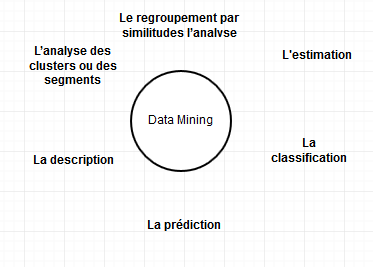
\includegraphics[scale=0.80]{application_word.PNG}
     \caption{Quelques tâches principales du Data Mining}
     \label{conceptsdm}
\end{figure}

Chaque tâche regroupe un ensemble de technique et de méthodes. C'est à l'utilisateur de choisir quelles techniques ou méthodes correspondent le mieux à son problème. Pour cela il faut faire une analyse au préalable de son jeux de données en identifiant par exemple quelles sont les variables discrètes \footnote{Variable discrète: Nombre fini de valeurs entre deux valeurs quelconques. Une variable discrète est toujours numérique} et variables continues\footnote{Variable continue:Nombre infini de valeurs entre deux valeurs quelconques. Une variable continue peut être numérique ou il peut s'agir de données de date/d'heure}. Ceci permet d'avoir non seulement un résultat efficace mais aussi facilitera l'étape de la préparation des données.

\subsubsection{L'estimation}
L’estimation repose généralement sur des variables continues. A partir de certaines données en entrée, on utilise l’estimation pour obtenir la valeur d’une telle variable: taille, revenu, chiffre d’affaire d’un client.  \\
Dans la pratique, l’estimation est souvent utilisée pour effectuer une tâche de classification. Lorsque l’on souhaite connaitre la durée de vie d’un client, on peut construire un modèle d’estimation qui calcule la probabilité de radiation du client en fonction des données dont il dispose. L’approche par estimation a le grand avantage que les enregistrements individuels peuvent être ordonnés en fonction du résultat. \\ \\
Une autre approche (l’approche de classification) est de créer un modèle qui attribue à chaque client une note. Celle-ci peut être un nombre entre 0 et 1 ou une annotation alphabétique indiquant la probabilité de vie d’un client. Imaginons par exemple qu’une entreprise vendeur d’énergie propose une réduction de 10\% à 10000 clients. Si l’on utilise l’approche de classification et que 15000 clients sont identifiés au total, alors on ne pourra offrir la réduction qu’aux 10000 clients déjà prévu tirés au hasard parmi le nombre total de client identifiés. Par contre la note attribuée aux clients permet d’offrir l’offre aux meilleurs candidats. \\ \\
Les réseaux de neurones sont particulièrement bien adaptés aux tâches d’estimation. 
\subsubsection{La classification}
Elle permet de créer des classes, des catégories, des degrés etc. Elle consiste à analyser des éléments d’un objet nouvellement présenté afin de l’attribuer à une classe d’un ensemble prédéfini.
Elle peut s’appliquer à différents cas: \\
\begin{itemize}
\item L'examen des demandes d’assurance frauduleuses
\item L’affectation des mots clés aux articles tels qu’ils arrivent à la rédaction d’un journal
\end{itemize}
Les arbres de décisions et le raisonnement basé sur la mémoire sont des techniques bien adaptées à la classification.
\subsubsection{La prédiction}
La prédiction ressemble à la classification et à l’estimation, mais les enregistrements sont classés selon un certain comportement futur ou une valeur future estimée.  Dans leurs ouvrages publiés en 1997 sur le Data Mining, Micheal Berry et Gordon Linoff disent que « \textit{Toute technique utilisée pour la classification et l’estimation peut être adaptée à la prédiction au moyen d’exemples d’apprentissage ou la valeur de la variable à prédire est déjà connue, à partir de données historiques par exemple}» Celles-ci sont utilisées pour construire un modèle qui explique le comportement actuel observé. \newline

Nous retenons dans l’approche par prédiction que lorsque le modèle est appliqué aux entrées actuelles, le résultat est la prédiction d’un comportement futur.  On peut citer des exemples auxquels le modèle de prédiction peut s’appliquer: 

\begin{itemize}
\item La prédiction des clients qui vont disparaître dans les trois ou six prochains mois,
\item La prédiction des abonnés du téléphone qui vont commander un service à valeur ajoutée comme l’appel multiple ou le courrier vocal
\end{itemize}
Les arbres de décision, Les règles d’associations, les réseaux de neurones, le raisonnement basé sur la mémoire sont quelques techniques qui peuvent être adaptés à la prédiction. Le choix parmi ces techniques dépendra du type de la valeur à prédire, de la nature des données en entrée…

\subsubsection{La description}
La description est dans la plupart des cas l’approche la plus simple à mettre en œuvre. En quelque sorte il s’agit de décrire ce qui se passe dans une base de données complexe, qui permettrait de mieux comprendre les clients, les produits, et les processus qui sont à l’origine des données. L’approche par la description permet d’indiquer où il faut aller chercher les explications. 

\subsubsection{L'analyse des clusters ou des segments}
L’analyse des clusters consiste à segmenter un ensemble de données hétérogènes en un certain  nombre de sous-groupes, plus homogènes, ou clusters. Dans cette approche, il n’y a ni classes prédéfinies ni exemples. L’analyse des clusters peut être la première étape d'une étude de segmentation du marché: au lieu de chercher une règle quelconque comme « quel est le type de promotion auquel les clients répondent le mieux ?», on peut diviser la base des clients en segments de personnes ayant les mêmes habitudes de consommation et se demander ensuite quelle est la bonne promotion pour chaque segment. 

\subsubsection{Le regroupement par similitudes ou l'analyse du panier de la ménagère}
Le regroupement par similitude consiste à déterminer les variables qui vont naturellement ensembles. L’exemple type est la détermination de produits qui se retrouvent dans un même caddie de supermarché, d’où le terme « analyse du panier de la ménagère ».

\subsection{Etude des techniques \label{etude_technique}}
Dans cette section, nous parlons des techniques que nous allons tenter de mettre en œuvre pour atteindre notre objectifs. Nous avons choisi ces techniques parce que nous pouvons adapter plus facilement leurs implémentations et l'appliquer à notre problème. A part leurs implémentations, nous pouvons personnaliser notre propre modèle en mettant en place une sur couche de fonctionnalités.   
\subsubsection{Les réseaux de neurones \label{reseaux_neurone}}
Les réseaux de neurones sont généralement optimisés par des méthodes d’apprentissage de type probabiliste. Ils sont placés d’une part dans la famille des applications statistiques, qu’ils enrichissent avec un ensemble de paradigmes permettant de créer des classifications rapides (réseaux de Kohonen en particulier), et d’autre part dans la famille des méthodes de l’intelligence artificielle auxquelles ils fournissent un mécanisme perceptif indépendant des idées propres de l'implémentation, et fournissant des informations d'entrée au raisonnement logique formel \cite{reseaux}.\\ 

Les réseaux de neurones sont à la base de certaines techniques descriptives et de certaines techniques prédictives du Data Mining. Il existe plusieurs types de réseaux de neurones, le choix de celui-ci détermine les résultats qui seront obtenus. Cette étape constitue la partie la plus difficile dans la mise en œuvre d'un réseau de neurones. La figure \ref{reseaux} montre un exemple de réseaux de neurones simple où N correspond à la valeur du nœud, P le poids associé à la connexion entre le nœud x et le nœud observé et F la fonction de transfert associée au nœud observé. Le réseau de neurone peut avoir plusieurs variables cibles. La couche de sortie aura autant de nœud qu'il y a de variable cible. La prédiction sera faite sur les valeurs des variables cibles.

  \begin{figure}[h]
   \centering
   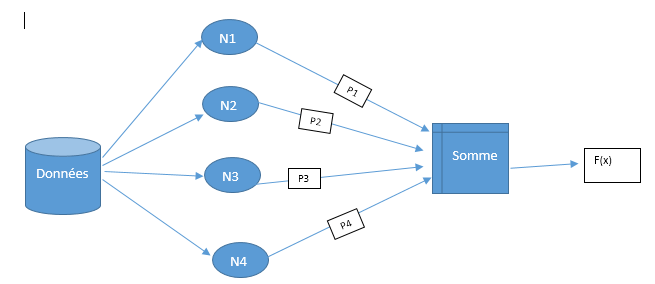
\includegraphics[scale=0.70]{structure_reseaux.PNG}
     \caption{Architecture du réseaux de neurone}
     \label{reseaux}
\end{figure}
\newpage
Généralement pour standardiser les valeurs, on utilise la formule du minimum et du maximum qui est la suivante:

\begin{equation}
  x= valeur - min(valeur)/max(valeur) - min(valeur)
\label{eq_1}
\end{equation}
 La formule \ref{eq_1} permet de standardiser les valeurs numériques. Ils existent d'autres moyens pour normaliser ce type de variables mais celle citée ci-dessus est plus intuitive. 
  

Connaissant pas comment les poids sont calculés exactement dans le réseau, nous allons essayer d'optimiser le résultat. Ainsi,  nous minimiserons les erreurs de prédiction en mettant en place un seuil. Ensuite nous comparons la valeur de sortie au seuil.\\\\

De façon générale, les étapes dans la réalisation d'un réseau de neurones pour prédire ou classer sont les suivantes: 
\begin{itemize}
\item L'identification des données en entrée et en sortie
\item La normalisation de ces données 
\item La constitution d'un réseau avec une structure adaptée
\item L'apprentissage du réseau 
\item Le test de réseau 
\item L'application du modèle généré par l'apprentissage
\item La dé-normalisation des données en sortie 
\end{itemize}

Rappelons que les données utilisées dans un réseau de neurones doivent être numériques et leurs valeurs doivent être comprises entre 0 et 1. \\

L'une des difficultés des réseaux de neurone est l'interprétation de ses résultats. Ces derniers sont difficiles à traduire et déployer au sein du service. La mise en place d'une telle technique nécessite beaucoup de temps. Par contre il est capable de gérer une grande quantité de donnée et prend en compte les données manquantes.

\newpage
\subsubsection{Les arbres de décisions}
La technique de l'arbre de décision est l'une des plus intuitives et des plus populaires du Data Mining. Elle supporte bien les données hétérogènes, manquantes et les effets non linéaires. Cette technique est employée dans la méthode de classement pour identifier des critères de données selon des classes prédéfinies. On commence par choisir la variable qui, par ses modalités sépare le mieux les données de chaque classe, de façon à avoir des sous-arbres que l'on appelle les nœuds \cite{stephane}. Ensuite, on réitère la même opération sur chaque nouveau nœud obtenu jusqu'à ce que la séparation des données ne soit plus possible. Le premier nœud de l'arbre est la racine. Les nœuds terminaux constituent les feuilles de l'arbre. Le chemin qui va de la racine à une feuille est l'expression d'une règle.
 \begin{figure}[h]
   \centering
   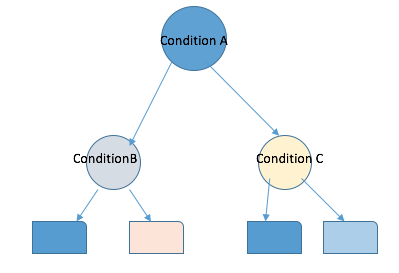
\includegraphics[scale=0.80]{arbre.png}
     \caption{Arbre de décision}
\end{figure}

Pour construire un arbre, il faut d'abord choisir la variable qui sépare le mieux les valeurs de chaque classe. Le nombre de condition de séparation dépend du type de variable. Par exemple lorsque la variable de séparation est de type binaire, nous n’aurons qu'une seule condition de séparation. Lorsque la variable est continue possédant n valeurs alors il y aura n-1 conditions de séparations. Le problème de construction d'un arbre réside généralement sur le choix de variable à chaque nœud et la condition de définition des branches. Ainsi lorsque l'on souhaite regrouper les entreprises par type de score (avec score= 1..9),  nous pouvons mettre en place un arbre de décision avec comme condition de séparation le score. L'autre alternative est d'utiliser une commande SQL pour interroger directement la base de données en faisant un GROUP BY. Le résultat produit par un arbre de décision est plus intuitif que celui produit par une requête SQL.
 Il existe plusieurs algorithmes pour mettre en place un arbre:

\subsubsection{CART(Classification And Regression Tree)}
Cette technique est la plus souvent adaptée à tout type de variable.
Sa généralité vient par le fait que le nombre de conditions de la variable à expliquer peut être fini ou non fini. Elle peut servir aussi au classement comme à la division. On retrouve cette méthode dans beaucoup de logiciels tels que SAS, R (rpart, tree)...
CART est capable de trouver la meilleure séparation des nœuds. Il permet aussi de calculer les coûts de mauvaise affectation en les intégrant dans le calcul de l'indice (où coéfficient) de Gini\footnote{L'indice de Gini: C'est une mesure statistique qui permet de mesurer des disparités dans une population donnée.}. Ce dernier est un critère de séparation pour tout type de variables explicatives \cite{gini}. C'est une fonction de pureté calculée ainsi. Par exemple selon 

\begin{equation}
  Gini(noeud)=1-\sum fi^2 
\end{equation}
où i= 1 à p, les fréquences relatives dans le nœud à prédire. Plus le nœud est pur, plus l'indice de Gini est moins élevé et inversement. 

\subsubsection{C5.0 de J.R Quinlan}
C5.0 est un arbre qui fonctionne en cherchant à maximiser le gain d'information réalisé en affectant chaque observation à une branche de l'arbre. Il partage avec CART son adaptation à l'étude de tout type de variables, sa recherche exhaustive de toutes les répartitions possibles ainsi que son dispositif d'optimisation de l'arbre par construction puis par découpage d'un arbre maximum. Il est implémenté sous R, SAS, IBM SPSS... 
 
\newpage

\section{Démarches \label{demarche}}
L’entreprise doit identifier les domaines où l’extraction des meilleures informations à partir des sources disponibles peut mener à une meilleure connaissance des actions à entreprendre. Lorsque ces ensembles d’actions sont bien identifiés, il faut les mettre en œuvre. Dans notre étude, nous partons sur l’hypothèse où les actions sont déjà définies.\\\\
Dans cette partie nous étudions la découverte des connaissances dirigées et non dirigées. Nous allons montrer en quoi consistent les deux démarches et comment les mettre en œuvre. Une grande partie de notre test a été réalisée sous R, Weka, et RapidMiner avec le même jeu de données. 
Ce sont ces logiciels qui sont à notre disposition au moment où nous écrivons ce mémoire. 
\subsection{La découverte des connaissances}
La découverte de connaissances est un processus permettant d'apprendre de nouvelles informations à partir d'une quantité massive de données dont on dispose. \\
Tout d'abord, nous montrons dans la figure \ref{figure10} en quoi consiste ce processus de découverte. Ensuite nous expliquons les deux catégories de découverte de connaissances qui sont: La découverte des connaissances dirigées et la découverte des connaissances non dirigées.

% * <lhillah@u-paris10.fr> 2016-06-19T09:30:37.596Z:
%
% > voir figure ci-dessous
%
% Il faut référencer explicitement la figure avec \ref{labelDeLaFigure}
%
% ^.
\begin{figure}[h]
\centering
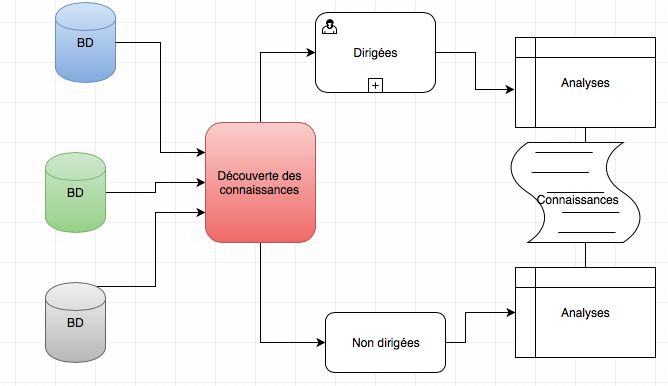
\includegraphics[scale=0.50]{kddnew.png}
\caption{Processus de découverte des connaissances}
\label{figure10}
\end{figure}

La Figure \ref{figure10} montre étape par étape la façon dont on peut découvrir des informations utiles à partir des bases de données. 
Après avoir recueilli les données, on décide si l'on doit diriger ou non la phase d'expérimentation. Généralement cette étape dépend de la nature des données et de l'objectif de l'analyse. 
Dans tous les cas, après l'identification des informations, une préparation des données est nécéssaire mais pas obligatoire. Il est intéressant de transformer les données pour avoir un meilleur resultat. Cela devient important lorsque l'on expérimente les mêmes données sur différents outils.
\subsubsection{Préparatin des données}
Il s'agit de consolider et nettoyer les données après avoir identifier les sources. Par exemple on vérifie si notre jeu de données contient des valeurs manquantes ou incorrectes à travers une fonction sur R (voir section \ref{log_dm}).  
Lorsque la fonction parcourt les données, s'il trouve une valeur manquante alors elle affiche le nombre de valeur manquante. Sinon elle mets zéro lorsqu'une valeur est présente avec la formule  \ref{valeur_manquante}.  
\begin{equation}
apply(data,2,function(x) sum(is.na(x)))
\label{valeur_manquante}
\end{equation}
La figure \ref{figure11} montre le résultat avec verification. 
\begin{figure}[h]
\centering
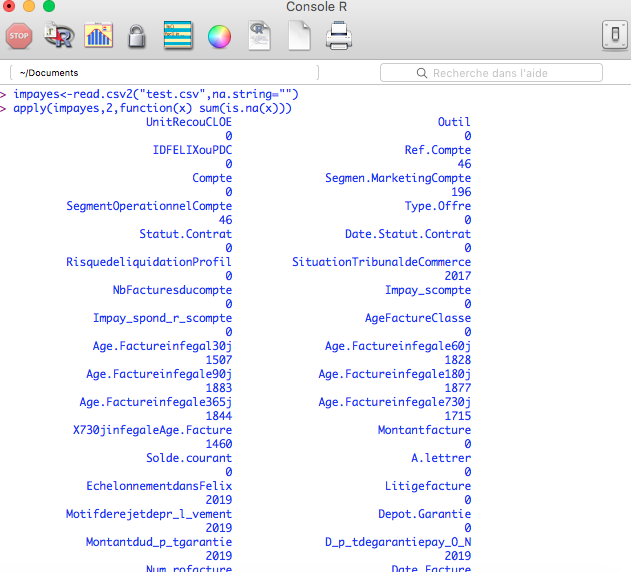
\includegraphics[scale=0.35]{manquantes.png}\\
\label{figure11}
\caption{Vérification des valeurs}
\end{figure}

On remarque que notre base contient quelques valeurs manquantes. C'est le cas de la variable "Segmentation opérationnelle Compte" dont la valeur à la ligne 46 est vide. Dans ce cas, soit nous supprimons toutes les valeurs manquantes, soit on les normalise.\\

La préparation des données ne se limite pas seulement à la suppression ou normalisation des données, il existe d'autres facteurs qui peuvent influencer le résultat généré par le modèle. Parmi ces facteurs on peut citer: l'existence des valeurs incomplètes ou erronées, le non prise en charge des caractères spéciaux dans les valeurs.

Cependant, lorsque l'exploration des données porte sur un ensemble de données très grandes, il est plus facile d'utiliser un outil de filtrage de données (SQL, ETL...).
Certains outils d'exploration de données proposent des ETL pour résoudre facilement des problèmes d'intégration de données.    


\subsection{La découverte des connaissances dirigées}

La découverte des connaissances dirigées, comme son nom l'indique consiste à expliquer la valeur d'une variable en fonction des autres variables:
\begin{itemize}
\item Quels sont les clients avec un gros montant dont le SIREN est radié ?
\end{itemize}
Comme le montre la Figure \ref{supervise}, l'utilisateur sélectionne une variable cible,  par exemple le "nombre de factures du compte" et il fait appel à un modèle d'apprentissage pour faire des estimations, des prédictions en fonction des autres variables (Age de la facture, montant, classe client...).  

Il consiste généralement à réaliser des tâches de classification (nous connaissons l'entrée et nous souhaitons déterminer la sortie) ou de régression (nous connaissons la sortie et nous souhaitons trouver l'entrée).  


\begin{figure}[h]
\centering
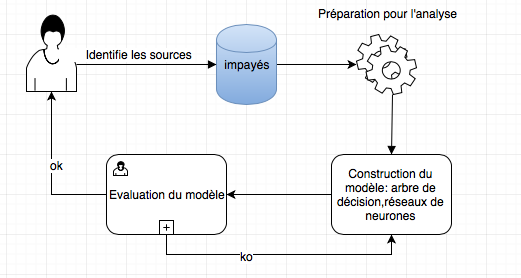
\includegraphics[scale=0.70]{dirigees.png}
\caption{Apprentissage supervisé}
\end{figure}
\label{supervise}
\newpage
\subsection{La découverte des connaissances non dirigées}
Dans la découverte des connaissances non dirigées, on ne précise pas de champ cible. C'est le modèle lui-même qui analyse librement les données. Elle s'applique lorsqu'on possèd un ensemble d'observations et que l'on souhaite extraire des informations intéressantes (recommandation, regroupement...) de façon automatique à partir de ses observations.\\\\
\begin{figure}[h]
\centering
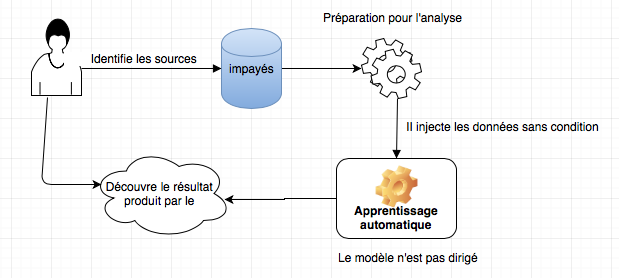
\includegraphics[scale=0.70]{nondirigees.png}
\caption{Apprentissage non supervisé}
\label{nondirigee}
\end{figure}
\newpage 

\section{Mise oeuvre de la solution \label{mise_en_oeuvre}}
Après avoir expliqué notre démarche sur la façon dont il est possible de tirer profit des informations, nous allons mettre en œuvre les techniques et d'analyser les résultats obtenus à travers ces dernières. 
  \subsection{Etude de cas : Analyse des impayés}
  
La mise en œuvre des techniques de Data Mining peut être réalisée de plusieurs manières selon le contexte, le secteur d'activité ou le résultat attendu. \\
Dans ce chapitre, nous allons appliquer les deux techniques expliquées dans la section \ref{etude_technique} page \pageref{etude_technique} à notre  jeu de données pour essayer de découvrir des informations utiles et pertinentes permettant d'améliorer la politique de gestion des impayés. Il s'agit des informations qui peuvent créer de la valeur ajoutée mais qui ne sont pas forcement détectables rapidement par l'être humain.
\\
Le but de cette expérimentation est d'analyser les impayés clients  en mode apprentissage dirigé et non dirigé  pour tester la faisabilité de notre approche et afin d'aider les analystes à capter les informations de façon rapide et efficace.

\subsection{Données \label{jeux_données}}  
 Notre jeu  de données concerne les clients professionnels. C'est un fichier plat au format CVS qui contient environ cinq cent mille observations (enregistrements) pour 76 variables. Ces variables constituent des informations clés comme par exemple: montants, l’âge de la facture, client sensible, la classe client... Pour des soucis de confidentialités, nous gardons l'anonymat de quelques variables.  \\
 La Figure \ref{donnees} montre une capture du fichier contenant l'ensemble des clients qui sont en situation d'impayés à une date données. Les clients sont regroupés par unité de recouvrement à laquelle ils sont rattachés. Bien évidemment, ces données évoluent dans le temps. Elles sont régulièrement mises à jour et analyser pour les analystes.  

     \begin{figure}[h]
% * <lhillah@u-paris10.fr> 2016-08-17T09:07:50.109Z:
%
% >      \begin{figure}[h]
% >    \centering
% >    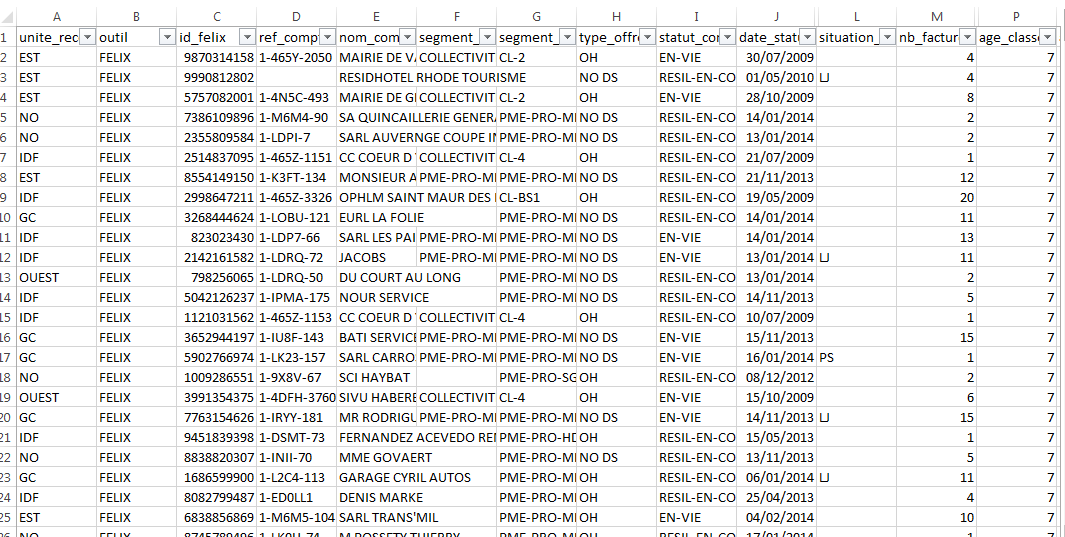
\includegraphics[scale=0.40]{donn_es.PNG}
% >      \caption{Jeu de données}
% >      \label{donnees}
% > \end{figure}
% > La Figure \ref{donnee
%
% Cette figure déborde dans la marge. Revoir son placement. Ou alors faire un vrai tableau (2 tableaux donc) à la place.
%
% ^.
   \centering
   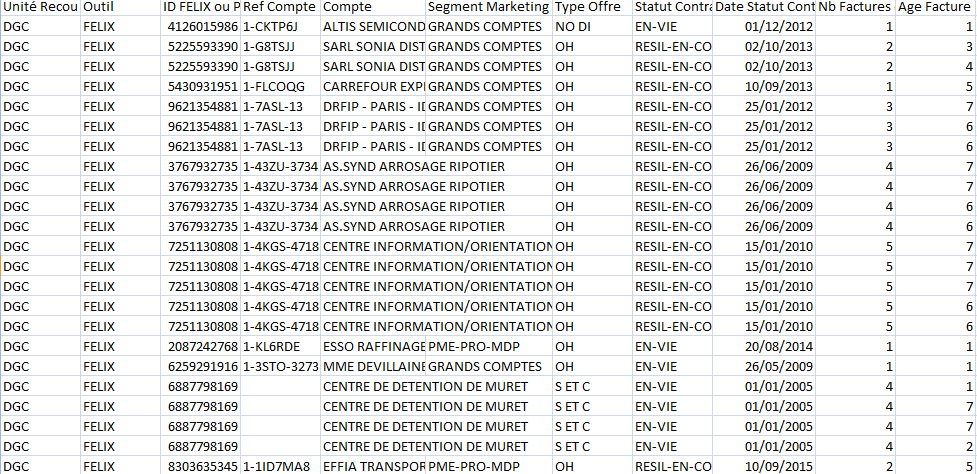
\includegraphics[scale=0.60]{jd1.PNG}
     \caption{Jeu de données}
     \label{donnees}
\end{figure}
\newpage


\subsection{Construction d'un arbre de décision}
Nous procédons à notre expérimentation en utilisant un arbre de décision. Nous avons choisi d'implémenter cette technique parce qu'elle est capable de gérer des données hétérogènes et offre un résultat lisible par les analystes. 
Nous allons diviser les données en deux échantillons. Le premier, l'échantillon d'apprentissage est utilisé pour construire le modèle. Le second, l'échantillon de test sera utilisé pour mesurer l'efficacité du modèle. Le but est de créer un modèle de décision qui classe l'âge de la facture du client en fonction du nombre de facture du compte. \\

Ainsi nous avons procédé de la manière suivante pour implémenter l'arbre: 
\begin{itemize}
\item Chargement du package (Party)
\item Chargement du jeu de données
\item Nous précisons les variables d'entrées et de sorties
\item Ensuite nous passons ces variables dans la fonction (ctree) avec les différentes paramètre(entrée,sortie)
\item La fonction "ctree" se chargera de la construction de l'arbre
\end{itemize}

Il faut noter ici que nous sommes pas obligés de préciser la variable de sortie. \newpage
La Figure \ref{figure15} montre un aperçu sur la règle de construction de l'arbre. Nous avons spécifié comme variable cible "l'âge de la facture" et la variable dépendante ici est "Nombre de factures du compte". 

\begin{figure}[h]
   \centering
   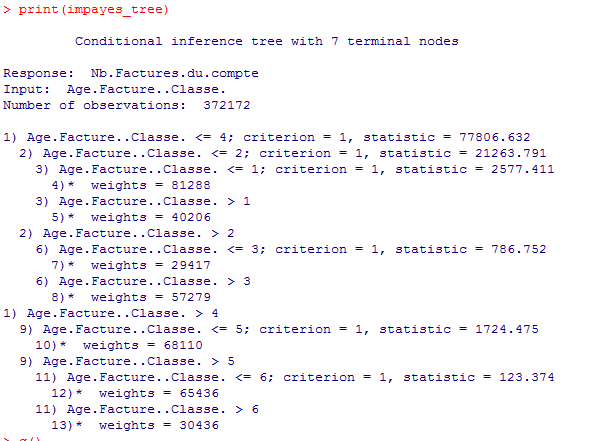
\includegraphics[scale=0.83]  {nbFacturecompte_age_factureclasse_tree_condition.PNG}
     \caption{Affichage de la règle de génération de l'abre}
     \label{figure15}
 
\end{figure}
Le premier sommet est appelé la racine de l'arbre et se situe sur le premier niveau. La première variable utilisée est la variable "Age.facture.Classe". Elle est composée de six valeurs (4;2;5;1;3;6) 
Au départ, nous constatons qu'il y a 372172 observations, quatre niveaux, cinq sous arbres et sept feuilles.  
\newpage
\subparagraph{Resultats:}
La Figure \ref{figure16} montre la création d'un arbre de décision à partir des règles générées par le modèle lui-même. En entrée, nous avons injecté l'âge de la facture ensuite le modèle crée des sous arbres en fonction du nombre de facture du compte. Il s'agit du résultat final qui doit être analysé par la suite par l'utilisateur.

\begin{figure}[h]
   \centering
   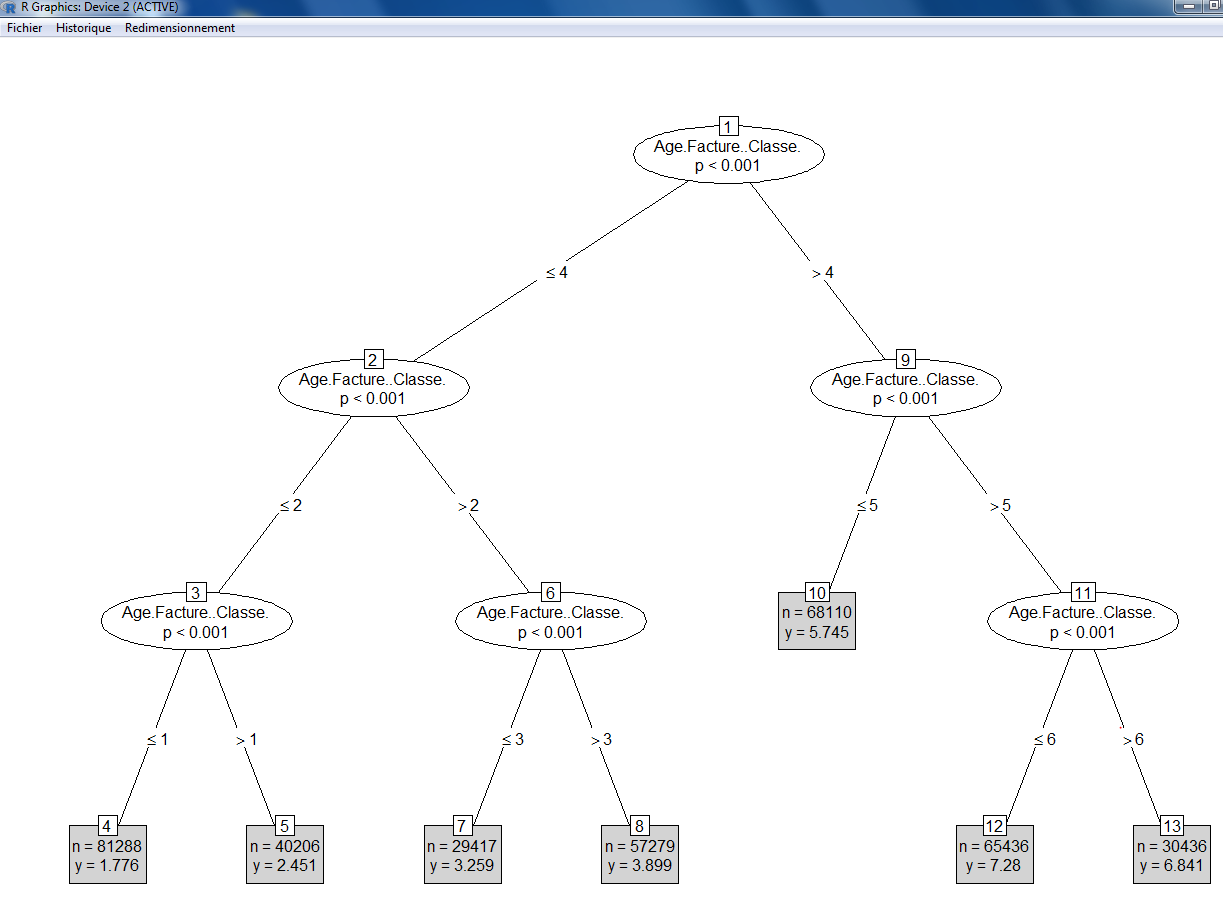
\includegraphics[scale=0.45]{ageclassenbfaturesimple_tree.PNG}
     \caption{Résultat}
     \label{figure16}
\end{figure}
\newpage
On remarque la classification de l'âge de la facture selon le nombre de facture du compte lié à un client. 
\begin{enumerate}
\item Le premier sous arbre  à droite est créé à partir de la condition "Age.Facture.Classe" >4 et <=5. Ce sous arbre couvre 68110 observations avec un taux d'erreur de 5.75\%.

\item Le sous arbre situé au niveau 3 à gauche correspondant à "Age.Facture.Classe" <=2 et <=1 couvre environ 82300 observations, soit un taux d'erreur de 1.8\%.
\end{enumerate}

On constate que les 372172 observations sont toutes distribuées:
\begin{equation}
          372172=81288+40206+29417+57279+68110+65436+30436
\end{equation}



\subsection{Construction à partir d'un réseau de neurone}
Cette solution suit à peu près la même démarche que la précédente. Dans un réseau de neurones, on peut injecter plusieurs variables. Cette fois, nous optons pour le mode d'apprentissage non dirigé, c'est à dire que le modèle sera généré sans condition à partir d'un échantillon de test. Nous choisissons ce mode d'apprentissage parce que nous souhaitons découvrir des relations intéressantes entre les valeurs. L'avantage de cette approche est qu'elle permet de tirer des résultats intéressants qui ne sont pas dans le périmètre de la politique. Nous voulons découvrir comment ces valeurs seront reparties entres elles. Les analystes pourront s'appuyer sur des découvertes pour anticiper des actions futures.     
 
\subsection{Construction du modèle} \label{page}
Nous allons utiliser le même jeux de données que dans la section \ref{jeux_données} page \pageref{jeux_données}. Nous avons choisi volontairement quelques variables parmi les 76. Parmi ces variables nous avons: Statut du contrat, et risque de liquidation. Nous allons tenter de mettre en œuvre les clients qui vont faire faillite en fonction de leur âge du nombre de facture et de l'âge de la facture. 
En entrée, nous avons les deux variables: le nombre de facture et l'âge de la facture que nous injectons dans le réseau. Notre variable cible est le score qui sera attribué aux clients. L'objectif est de surveiller les clients qui risquent de faire défaillance.\\
Pour des problèmes de cohérence de données, nous avons normalisé toutes les valeurs sous forme numérique. Cela permet d'avoir un meilleur résultat.   
Après avoir terminé l'étape du choix des variables pour le test, nous allons appliquer l'algorithme sur les données (Figure \ref{figure18} ci-dessous).
\newpage


    \begin{figure}[h]
% * <lhillah@u-paris10.fr> 2016-08-17T09:09:05.398Z:
%
% >     \begin{figure}[h]
% >    \centering
% >    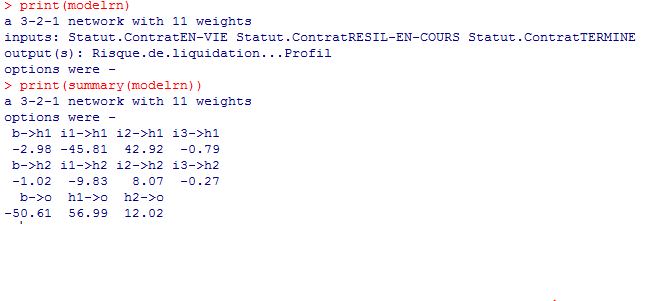
\includegraphics[scale=0.7]{neural.PNG}
% >      \caption{Réseaux de neurones}
% >      \label{figure18}
% > \end{figure}
%
% Illisible, aggrandir ou trouvez une autre forme que cette figure pour présenter l'information.
%
% ^. fait
   
   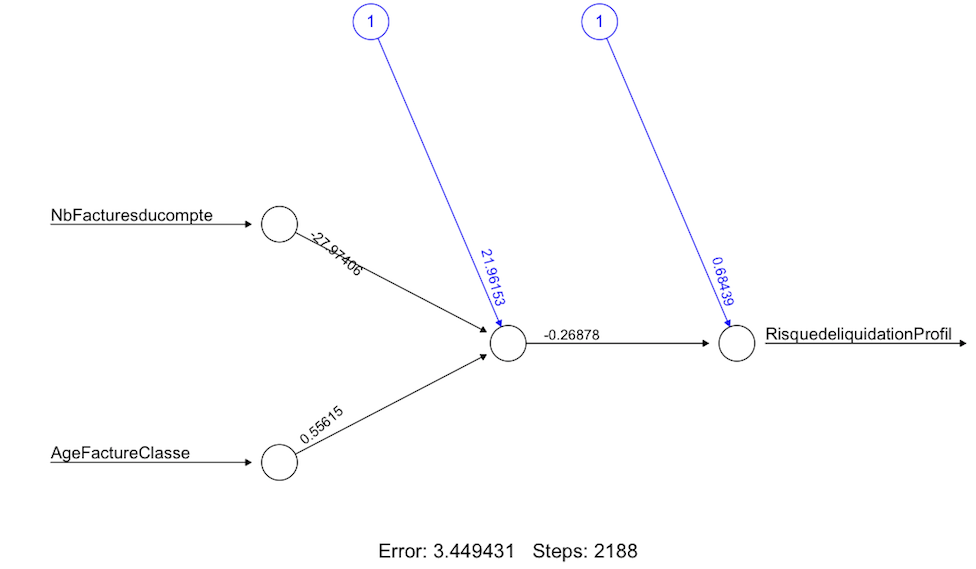
\includegraphics[scale=0.45]{neural1.png}
     \caption{Réseau de neurone simple}
     \label{figure18}
\end{figure}
Ce test a été effectué sur un échantillon de donnée que nous avons généré aléatoirement. Voici les étapes: 

\begin{itemize}
\item index <- sample(1:nrow(data),round(0.75*nrow(data)))
\item train <- data[index,]
\item test <- data[-index,]
\end{itemize}
La Figure \ref{figure18} calcule la probabilité de score d'un client en fonction du nombre de facture et son âge de facture. Nous voyons également le taux d'erreurs (3,449) associé au résultat  et le nombre d'étape. Cette dernière constitue les opérations effectuées au sein du réseau. \\\\
Plus la taille du jeu de données est grande plus le réseau donne un meilleur résultat. La figure suivante \ref{neural2} montre cette différence.
 
\newpage
\begin{figure}[h]
   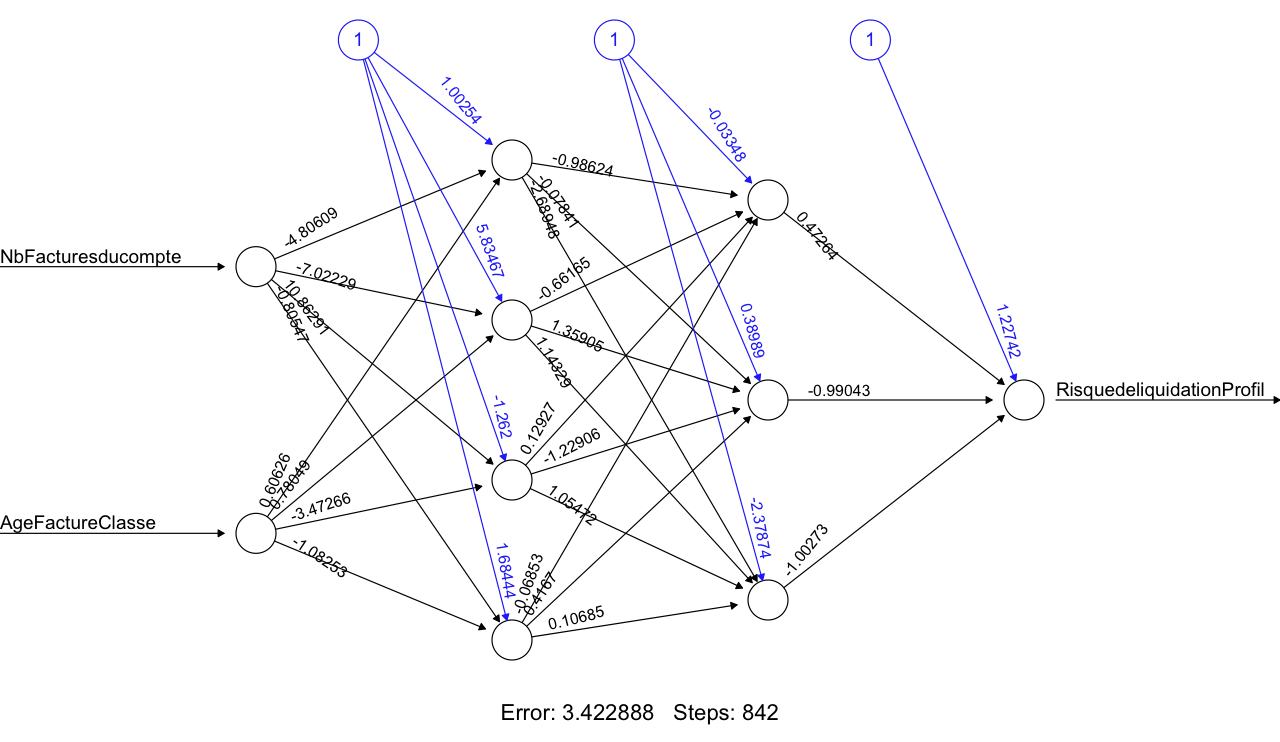
\includegraphics[scale=0.36]{neural2.png}
     \caption{Réseau de neurone avec plusieurs sous couches}
     \label{neural2}
\end{figure}

Nous remarquons une légère baisse du taux d'erreurs qui est passé de 3,449 à 3,23 et l'apparition de plusieurs sous couches.
Comme expliquer dans la section \ref{reseaux_neurone} page \pageref{reseaux_neurone} plus le nombre de sous couche est important plus le résultat devient de plus en plus fiable. 
Nous avons procédé de la façon suivante: 
\begin{itemize}
\item Transformation des données: cette étape n'est pas obligatoire 
\item Chargement des données 
\item Chargement des packages nécessaires à la réalisation du réseau
\item Normalisation des valeurs en utilisant la méthode min-max
\item Choix du type d'algorithme (neuralnet)
\item Application de l'algorithme aux données 

\end{itemize}
 La méthode de normalisation "min-max" est une technique facile qui permet d'adapter ses données en fonction des opérations que nous souhaitons réaliser. Il existe d'autres méthodes de normalisation comme "Z-nomalization" mais notre choix a été porté sur celui de Min-Max parce qu’il est bien compatible et facile à mettre en place sous R. Le tableau \ref{temps} ci-dessous montre le délai de traitement en fonction de la quantité de données sur R. 


 \begin{table}

 \begin{tabular}{|M{4cm}|M{5cm}|M{5cm}|} 
\hline  
   Nombre de ligne & Temps de traitement & Résultat\tabularnewline  
\hline 
< 100000  & Instantané & On voit tout de suite le résultat  \tabularnewline  
\hline 
 > 100000 et <500000 & Marche partiellement. Lorsque nous rejouons plusieurs fois les opérations, R plante car la mémoire allouée a été dépassée ou atteinte & Dans la plupart des cas le résultat n'est pas affiché  \tabularnewline  
\hline 
  >=500000 & Lorsque l'exécution est lancée, elle reste bloquer pendant un certain moment  & Le résultat est rarement obtenu  \tabularnewline
\hline 
 
\end{tabular}
\caption{Temps de traitement sur R 3.3}
\label{temps}
\end{table}
\newpage
Malgré la diversité de technique que propose R, il peut poser des problèmes en terme de performance comme expliquer dans la section \ref{log_dm} page \pageref{comparai_logiciel}. Il existe des alternatives pour contourner ce problème sur R que nous allons expliquer dans la section suivante.

\subsection{Évaluation}
% * <lhillah@u-paris10.fr> 2016-08-17T08:50:11.563Z:
%
% > Évaluation
%
% Ce n'est pas assez fouillé. Il faut d'abord annoncer les critères, puis réaliser l'évaluation selon ces critères, avec vos commentaires personnels.  Faire une synthèse en indiquant dans quel cas telle technique s'appliquerait mieux que telle autre
%OK
% ^.
Après avoir présenté les deux techniques possibles permettant de mettre en œuvre l'apprentissage supervisé et non supervisé, nous allons comparer notre approche et l'approche d'avant afin de montrer les points négatifs et positifs de chacune d'elles. D'un point de vu métier notre objectif est de permettre aux analystes d'avoir une vision globale sur l'ensemble des portefeuilles clients et à faciliter les processus de gestion de créances clients. Actuellement, ils n'ont pas cette vision de fouille de données. Notre approche apportera non seulement une amélioration dans le traitement de données mais aussi une optimisation des méthodes existantes de gestion de risque en automatisant des tâches répétitives. Souvent, les analystes ont des problématiques sur la gestion des clients tels que le suivi des impayés des sociétés qui n'existent plus mais ils ne savent pas comment les mettre en place. Ainsi ils peuvent s'appuyer sur notre approche pour surveiller en parallèle de leurs tâches quotidiennes les clients à fortes risques pour anticiper des actions futures. Le tableau \ref{metier} compare la différence entre l'approche d'avant et notre approche en fonction des objectifs \\\\

\newpage
\begin{table}

\begin{tabular}{|M{4cm}|M{4cm}|M{4cm}|} 
\hline  
    & L'approche d'avant& Notre approche\tabularnewline  
\hline 
Gain de temps & ++ & +++ \tabularnewline  
\hline 
  Traitements exhaustifs des données & ++ & +++ \tabularnewline
\hline 
Automatisation des tâches & ++ & +++ \tabularnewline
\hline 
Interprétation des résultats & +++ & + \tabularnewline
\hline 
Coûts & Gratuit. Une partie des tâches est sous-traité (payant)  & Demande des ressources humaines et matérielles.  \tabularnewline
\hline 
Maintenance & Très rarement & Généralement, la maintenance est faite en fonction de l'évolution des bésoins. \tabularnewline
\hline 
\end{tabular}
\caption{Tableau comparatif des approches}
\label{metier}


\end{table}

D'un point de vue technique, notre approche peut traiter exhaustivement les données dans un temps raisonnable contrairement à l'approche d'avant. Les techniques testées dans ce mémoire permettent de faciliter le classement et la mise en relation des données homogènes ou hétérogènes. Dans la section précédente, nous avons constaté des problèmes de traitement de données de grande taille sur R. En général, ceci peut poser un frein dans la mise en place des techniques de Data Mining dans le contexte actuel ou le traitement de gros volume de données fait partie des enjeux des grandes entreprises. Selon notre cas, nous pouvons faire recours à d'autres logiciels de Data Mining capables de résoudre ce problème comme le logiciel commercial SAS. Il s'agit dans un premier temps de charger les données sur SAS, ensuite nous lirons directement les données à partir des tables SAS via le package "foreign" de R.   \\
La première technique expliquée, l'arbre de décision, repose sur l'utilisation des règles. L'avantage de cette solution est que les règles peuvent être facilement exprimées dans un langage de bas niveau ou dans un langage de type SQL. Ainsi on est capable de calculer le taux d'erreur de l'arbre de décision pour estimer le niveau de confiance du modèle ou en sélectionnant le meilleur sous arbre. C’est une des rares méthodes que l’on peut présenter assez rapidement à un public non spécialiste du traitement des données sans se perdre dans des formulations mathématiques délicates à appréhender. Cette technique peut être mise en œuvre lorsque nous souhaitons réaliser des tâches de classement ou d'estimation par exemple. \\
Par contre, cette solution présente des limites. Dans de nombreux cas, elle ne peut traiter que des valeurs binaires (1/0, Oui/Non). Cette solution est couteux en terme calcul car au niveau de chaque nœud un tri est fait pour trouver la meilleure orientation d'un sous arbre. Dans le contexte actuel, il sera difficile de déployer cette solution car sa mise en œuvre demande plusieurs ressources (humaines, matérielles). Dans un secteur comme l'énergie, cette technique a sa place dans les services qui s'occupent des créances clients car elle leurs permet par exemple d'analyser très vite le risque de solvabilité des clients.\\\\
Concernant la deuxième technique, le réseau de neurone, elle permet de calculer une valeur estimée (la sortie) à partir des valeurs d'entrées. Le réseau de neurone fonctionne mieux lorsque toutes les valeurs d'entrées sont comprises entre 0 et 1. L'utilisation de cette technique est recommandée lorsque nous avons des idées en tête mais nous ne savons pas comment les réaliser. Cette technique est déjà utilisée dans d'autres secteurs comme le secteur de l'assurance pour lutter contre les fraudes. Dans notre contexte, elle est applicable par exemple dans le cadre des recherches du suivi de paiements de factures. Les analystes seront en mesures de connaître et d'identifier facilement les clients susceptibles de ne pas payer dans le délai. \\
Cependant, l'adoption de cette démarche nécessite une transformation non négligeable des données. Il s'agit de normaliser les valeurs d'entrées et de sorties. Il est difficile de connaître comment les données sont calculées à l'intérieur d'un réseau de neurone. Cela peut impacter la compréhension des résultats produits. Nous avons rencontré des difficultés lors de la mise en place de cette technique. Premièrement, la compréhension de la  technique en elle même nécessite du temps et d'investissement. Il faut comprendre comment elle est construite  et sur quoi elle se base réellement pour faire ses calculs. Deuxièmement, il est difficile d'interpréter ses résultats. \\
Cependant, nous pouvons élargir notre approche en ajoutant des tâches supplémentaires. Après avoir mis en place les techniques, nous allons créer un formulaire  qui servira d'interface entre le métier et l'ensemble des processus techniques. Cela rendra facile la prise en main et l'utilisation des techniques de Data Mining.\\\\
La prochaine étape que nous avons pas pu mettre dans ce mémoire est la mesure des qualités de nos résultats en utilisant les notions de Precision\footnote{Precision: Precision: C'est le nombre de réponses pertinentes données/nombre de réponses données}/Recall\footnote{Recall: C'est le nombre de réponses pertinentes données/nombre de réponses pertinentes existant}. Ces notions sont importantes dans notre contexte car elles expriment le point de vue du métier. Par exemple elles mesurent le degré de satisfaction des utilisateurs au cas où  ces derniers devront lire des informations qui ne les intéressent pas.

\newpage
\section{Bilan \label{bilan}}
Avant de conclure ce mémoire, nous allons établir le bilan de notre recherche avec des avantages et des limites.   
\subsection{Avantages}
Notre recherche sur les techniques de Data Mining montre que cette démarche est une étape essentielle pour les systèmes d'aide à la décision d'une entreprise ou les données et les chiffres sont au cœur du métier. Elle permet de générer des idées qui seront ensuite vérifiées à l'aide d'approche plus dirigée. \\

L'un des avantages du Data Mining est l'analyse de gros volumes de données (des millions de données) parfois en temps réel. En effet, il est possible de découvrir des formes et des relations intéressantes qui peuvent aider les utilisateurs  à entreprendre de nouvelles actions.\\

De plus, le Data Mining est lié à plusieurs disciplines comme le business intelligence, la Data visualisation... La découverte des connaissances  à partir des données d'une entreprise est une source de valeur qui donne un avantage concurrentiel. Grâce à elle, on peut se baser sur les évènements du passé pour prédire les évènements du futur et aussi en améliorant la compréhension des clients. \\


\subsection{Limites}
Il est évident que les solutions de Data Mining présentent un avantage majeur dans les systèmes d'aide à la décision. Cependant, est-il facile de mettre en place une solution de Data Mining au sein d'une entreprise ? \\

A travers notre expérience, nous avons remarqué qu'il est difficile de trouver la meilleure technique à appliquer aux problèmes. Certains algorithmes ne traitent que des valeurs binaires. Ces techniques de Data Mining ne sont pas faciles à mettre en place pour plusieurs raisons. La personne qui implémente les techniques doit avoir un minimum de connaissance en statistique et mathématique. Il y a aussi le choix du bon logiciel en fonction de ses contraintes.  \\

On a remarqué aussi que l'une des limites des techniques du Data Mining est l'interprétation des résultats. Généralement, les résultats produits sont souvent difficile à traduire. Par exemple, un nombre important de variables dans un réseau de neurones fait qu'il produit des résultats assez complexes. Malheureusement, nous n'avons pu évaluer la qualité des résultats fournis par l'approche d'avant et notre approche.



\newpage
\section{Conclusion \label{conclusion}}
Nous avons étudié à travers ce mémoire des techniques de Data Mining ainsi que leurs applications dans la finance de marché du secteur de l'énergie. Nous avons expliqué aussi les concepts de Data Mining dans le but de résoudre notre problème par des solutions que propose le Data Mining. Malgré l'efficacité des techniques de Data Mining et son application dans de nombreux domaines, il n'est pas facile d'intégrer une telle démarche dans un environnement ou la qualité et la précision des résultats sont importants. En effet, il est nécessaire de maîtriser toutes les sources d'informations et de comprendre le métier.\\

Bien attendu, nous n'avons abordé qu'un seul problème et nous avons cherché à le résoudre de façon méthodique. Nous avons mis en œuvre deux techniques de Data Mining qui sont généralement les plus efficaces pour découvrir et élargir notre périmètre de compréhension sur la gestion des risques. D'autres techniques et solutions de Data Mining  plus récentes peuvent améliorer la performance et faciliter la mise en œuvre des concepts. \\

Les techniques de Data Mining peuvent apporter une amélioration dans les systèmes d'aide à la décision. Lorsque cette amélioration est réelle, faut-il intégrer toute la démarche du Data Mining au sein de l'entreprise? Nous nous demandons alors s'il faut aller plus loin sur la mise en place des techniques de Data Mining? Peut-on connecter directement les outils de Data Mining aux outils Big Data?

 \newpage
 \bibliographystyle{plain}
\bibliography{bibliography.bib}
\addcontentsline{toc}{chapter}{Bibliographie}
\newpage
%\addcontentsline{toc}{chapter}{Annexe}
%\appendix\section*{Annexe}
\end{document}